% ─── Section 1: Introduction ──────────────────────────────────────

\section{Introduction}
\label{sec:intro}

Volatility targeting (VT), the practice of dynamically scaling portfolio exposure inversely to predicted volatility, has attracted considerable attention following the influential work of \citet{moreira2017}. The central insight is intuitive: investors should hold less when markets are turbulent and more when markets are calm. Studies have documented that this approach reduces maximum drawdown substantially, though its impact on risk-adjusted returns remains debated \citep{fleming2001,harvey2018}.

Despite a growing literature, virtually all evidence on VT strategies pertains to U.S. markets or, more broadly, to developed Western economies. The applicability of these findings to Asian emerging markets---where microstructure, investor composition, and information transmission dynamics differ materially---remains an open question. This gap is particularly surprising in the case of Taiwan, which ranks among the world's most active equity markets by turnover ratio, hosts a retail-investor-dominated trading environment where individual investors account for over 60\% of turnover \citep{barber2009}, and features extreme single-stock concentration: Taiwan Semiconductor Manufacturing Company (TSMC) alone constitutes approximately 50\% of the benchmark 0050.TW index. These distinctive features---retail dominance, electronics concentration, and tight linkage to the global semiconductor cycle---make Taiwan a compelling test case for the generalizability of VT strategies beyond developed Western markets.

The Taiwan stock market presents several features that make it a compelling laboratory for VT research in the emerging-market context. First, the TAIEX exhibits a leverage effect---the asymmetric volatility response to positive and negative shocks formalized by \citet{black1976} and \citet{glosten1993}---that is substantially stronger at the index level than at the individual stock level. We document that this \textit{diversification amplification} reaches approximately 5.0$\times$ for the broad TAIEX ($\sim$900 stocks) relative to nine individual stocks (90\% bootstrap CI: $[2.8, \, 8.1]$), though a more modest 1.6$\times$ for the investable 0050.TW ETF (50 stocks), compared to 2.8$\times$ in the United States, a difference we attribute to higher correlation asymmetry among Taiwanese equities during market declines \citep{ang2002}. Second, the absence of a deep, liquid local implied volatility index (the VIXTWN was introduced only in November 2020 with limited history) forces practitioners to rely on either model-based volatility estimates or proxy measures such as the U.S. VIX \citep{whaley2000,whaley2009}---a constraint common to many emerging markets. The viability of this proxy approach has broader implications for VT implementation across markets where implied volatility surfaces are underdeveloped, analogous to the cross-listing and ADR literature that documents how U.S.-listed securities transmit price information to local markets \citep{gagnon2010}. Third, Taiwan's geographic position---trading hours that open after the U.S. market closes---creates a natural information transmission channel \citep{eun1989,hamao1990,lin1994} that provides supplementary evidence for cross-market price discovery (Appendix~\ref{app:tz}).

This paper makes three contributions.

\textbf{First}, we document the leverage effect and its diversification amplification in the Taiwan market, extending the analysis of \citet{ang2002} to an Asian emerging-market context. Using GJR-GARCH estimation on the TAIEX ($\gamma = 0.272$, $t = 3.18$), nine individual Taiwanese stocks, and the 0050.TW ETF ($\gamma = 0.087$), we show that the broad TAIEX gamma exceeds the average individual stock gamma by a factor of approximately 5.0$\times$ (90\% bootstrap CI: $[2.8, \, 8.1]$), though the investable 0050.TW (50 stocks) shows a more modest amplification of 1.6$\times$. This amplification arises because stock correlations increase asymmetrically during downturns, a phenomenon first identified by \citet{ang2002} for U.S. equities. We further establish a strong cross-market spillover channel: lagged SPY returns predict next-day 0050.TW returns with a correlation of $r = 0.376$, and VIX Granger-causes Taiwan equity volatility ($F = 58.8$, $p < 0.001$).

\textbf{Second}, we evaluate multiple VT strategies adapted for Taiwan, including EWMA-based VT, GJR-GARCH VT, and a VIX-proxy approach ($8.63/\text{VIX}$) calibrated using the VIXTWN-to-VIX ratio of 1.39. Over a common evaluation period (2020--2026), VT strategies improve both Sharpe ratios and maximum drawdowns relative to buy-and-hold, with GJR VT achieving the highest Sharpe (1.108). The EWMA strategy, evaluated over the longer 2010--2026 sample, improves the Sharpe ratio from 0.729 to 0.796 while halving maximum drawdown from $-41.3\%$ to $-18.4\%$. We show that Student-$t$ Value-at-Risk achieves a 0.5\% violation rate over 2020--2026, within the Basel III Green Zone (noting that the traffic-light framework is defined for 250-day windows; we apply the 1\% threshold as a benchmark across our full sample). A key finding is that despite the statistically significant leverage effect, GJR-GARCH does not significantly improve QLIKE over standard GARCH (Diebold-Mariano $p = 0.86$), yet GJR-based VT produces a meaningfully higher Sharpe ratio (+0.114), suggesting that tail-specific forecast accuracy---rather than average forecast accuracy---drives VT performance. A systematic cross-market validation reveals that three of four core U.S. VT findings generalize or partially generalize to Taiwan (VIX sufficiency, allocation near vol-parity, calendar null results), while one does not (rebalancing frequency), providing a nuanced picture of VT portability to emerging Asian markets.

\textbf{Third}, we exploit TAIFEX tick-level futures data to construct 5-minute realized volatility (RV) for Taiwan equity index futures, revealing three findings that fundamentally alter the model selection landscape. (a) HAR-RV \citep{corsi2009} crushes GJR-GARCH in volatility prediction (QLIKE improvement of 66\%, Diebold-Mariano $t = -11.14$), demonstrating that the daily r-squared ``proxy ceiling''---not a model ceiling---previously obscured meaningful differences among forecasting models. (b) Despite this prediction superiority, HAR-RV produces \textit{worse} Value-at-Risk coverage than GJR+Cornish-Fisher (17 violations vs.\ 2), establishing a ``prediction-VaR paradox'' wherein better volatility forecasts do not automatically translate into better tail-risk management. (c) Realized GARCH \citep{hansen2012}, which combines GARCH's conditional residual structure with RV-informed variance updating, partially resolves this paradox by achieving both Trinity PASS VaR coverage and the highest rank-order correlation (Spearman $\rho = 0.790$). We additionally show that TAIFEX night session returns account for 73.7\% of the total daily return and that 61\% of the overnight gap variance is tradable via the futures night session (regression $R^2 = 0.83$), challenging the conventional view that the overnight gap is an untradable risk.

We additionally document a cross-market information transmission channel---lagged U.S. returns predict next-day Asian equity returns, with approximately 78\% of the signal absorbed by the opening gap---presented as supplementary evidence in Appendix~\ref{app:tz}. This time-zone analysis, while related to the VIX-proxy motivation, constitutes a distinct microstructure contribution that we defer to supplementary material to maintain the paper's focus on VT strategy evaluation.

The remainder of the paper proceeds as follows. Section~\ref{sec:data} describes the data and methodology. Section~\ref{sec:leverage} examines the leverage effect and diversification amplification. Section~\ref{sec:vt} evaluates VT strategies, including a conditional leverage extension and futures implementation. Section~\ref{sec:hf} presents high-frequency volatility evidence from TAIFEX tick data. Section~\ref{sec:macro} explores macroeconomic indicators for Taiwan. Section~\ref{sec:var} addresses VaR and risk management. Section~\ref{sec:discussion} discusses practical implications and cross-market validation. Section~\ref{sec:conclusion} concludes. Appendix~\ref{app:tz} presents supplementary evidence on time-zone information transmission from U.S. to Asian equity markets.


% ─── Section 2: Data and Methodology ────────────────────────────

\section{Data and Methodology}
\label{sec:data}

\subsection{Data Sources}

We use daily closing prices, adjusted for dividends and splits, for the following instruments obtained from Yahoo Finance and the Taiwan Stock Exchange (TWSE):

\begin{itemize}
    \item \textbf{0050.TW}: Yuanta/P-shares Taiwan Top 50 ETF, tracking the FTSE TWSE Taiwan 50 Index. Sample: January 2008 to March 2026 (4,532 trading days).
    \item \textbf{TWII (TAIEX)}: Taiwan Capitalization Weighted Stock Index. Sample: January 1997 to March 2026 (7,148 trading days).
    \item \textbf{Nine individual Taiwan stocks and one ETF}: Taiwan Semiconductor (2330.TW), Hon Hai Precision (2317.TW), MediaTek (2454.TW), Cathay Financial (2882.TW), Mega Financial (2886.TW), CTBC Financial (2891.TW), Chunghwa Telecom (2412.TW), Yuanta Financial (2885.TW), Fubon Financial (2881.TW), and Yuanta High Dividend ETF (0056.TW, an ETF tracking mid-cap dividend stocks, included for completeness but excluded from the primary individual-stock average; see Section~\ref{sec:leverage}).
    \item \textbf{U.S. benchmarks}: S\&P 500 (SPY), CBOE Volatility Index (VIX), CBOE Emerging Markets ETF Volatility Index (VXEEM), and the iShares MSCI Taiwan ETF (EWT).
    \item \textbf{Asia-Pacific markets}: Nikkei 225 (Japan), Hang Seng (Hong Kong), ASX 200 (Australia), Straits Times (Singapore), KOSPI (South Korea), and Sensex (India).
    \item \textbf{VIXTWN}: TAIEX Options Volatility Index, compiled by the Taiwan Futures Exchange (TAIFEX) using the CBOE VIX methodology. Available from November 2020.
\end{itemize}

Log returns are computed as $r_t = \ln(P_t / P_{t-1}) \times 100$. Table~\ref{tab:summary_stats} reports summary statistics.

\begin{table}[H]
\centering
\caption{Summary Statistics for Key Assets}
\label{tab:summary_stats}
\begin{tabular}{lcccccc}
\toprule
& Mean (\%) & Std (\%) & Skewness & Kurtosis & $\gamma_{\text{GJR}}$ & $t(\gamma)$ \\
\midrule
TWII (1997--2026) & 0.019 & 1.45 & $-0.31$ & 5.82 & 0.272 & 3.18 \\
0050.TW (2008--2026) & 0.034 & 1.38 & $-0.47$ & 4.73 & 0.087 & 2.20 \\
SPY (2008--2026) & 0.042 & 1.18 & $-0.52$ & 12.30 & 0.211 & 5.79 \\
TSMC (2330.TW) & 0.051 & 1.92 & $-0.18$ & 3.41 & 0.039 & 0.87 \\
9-stock average (excl.\ 0056) & 0.026 & 1.74 & $-0.21$ & 3.62 & 0.054 & --- \\
10-security average (incl.\ 0056 ETF) & 0.028 & 1.71 & $-0.22$ & 3.68 & 0.060 & --- \\
\bottomrule
\end{tabular}
\begin{flushleft}
\small \textit{Notes:} $\gamma_{\text{GJR}}$ is the asymmetric leverage parameter from GJR-GARCH(1,1) with $w = 2000$ rolling window. $t(\gamma)$ uses Newey-West HAC standard errors. 0056.TW is itself a diversified ETF (30+ constituents) and is therefore excluded from the primary 9-stock average used in the amplification ratio calculation (Section~\ref{sec:leverage}). The 10-security average including 0056 is reported for completeness.
\end{flushleft}
\end{table}

\subsection{Volatility Models}

We employ three volatility models from the ARCH/GARCH family \citep{engle1982,bollerslev1986}, estimated via rolling-window quasi-maximum likelihood \citep{bollerslev1992}.

\textbf{GJR-GARCH(1,1)} \citep{glosten1993}:
\begin{equation}
\sigma_t^2 = \omega + (\alpha + \gamma \cdot \mathbb{1}_{r_{t-1}<0}) \, r_{t-1}^2 + \beta \, \sigma_{t-1}^2
\label{eq:gjr}
\end{equation}
where $\gamma > 0$ captures the leverage effect: negative returns increase conditional variance more than positive returns of equal magnitude.

\textbf{GARCH(1,1)} \citep{bollerslev1986}: the restriction $\gamma = 0$ of Equation~\eqref{eq:gjr}.

\textbf{EWMA (Exponentially Weighted Moving Average)}:
\begin{equation}
\sigma_t^2 = \lambda \, \sigma_{t-1}^2 + (1 - \lambda) \, r_{t-1}^2
\label{eq:ewma}
\end{equation}
with decay factor $\lambda = 0.94$, the default recommended by the RiskMetrics methodology \citep{jpmorgan1996}. EWMA requires no parameter estimation and can be implemented without optimization software.

All GARCH and GJR-GARCH models are estimated using a rolling window of $w = 2000$ trading days, following \citet{hwang2006} who demonstrate that windows below 500 induce substantial persistence bias. We verify that our core results are robust to $w = 504$ and $w = 1000$.

\subsection{Forecast Evaluation}

We evaluate volatility forecasts using the QLIKE loss function \citep{patton2011}:
\begin{equation}
\text{QLIKE}_t = \ln(\sigma_t^2) + \frac{r_t^2}{\sigma_t^2}
\label{eq:qlike}
\end{equation}
which is robust to noise in the volatility proxy $r_t^2$ and penalizes underprediction more heavily than overprediction. Model comparisons use the \citet{diebold1995} test with Newey-West standard errors for the null hypothesis of equal predictive ability.

\subsection{Volatility Targeting Strategies}

A volatility targeting strategy sets the portfolio weight as:
\begin{equation}
w_t = \frac{\sigma_{\text{target}}}{\hat{\sigma}_t}
\label{eq:vt}
\end{equation}
where $\sigma_{\text{target}}$ is the annualized target volatility and $\hat{\sigma}_t$ is the volatility forecast. The weight is capped at 100\% (no leverage). The portfolio return is:
\begin{equation}
r_t^{\text{VT}} = w_{t-1} \cdot r_t + (1 - w_{t-1}) \cdot r_t^{f}
\label{eq:vt_return}
\end{equation}
where $r_t^{f}$ is the risk-free return (proxied by the 3-month Treasury bill rate) and the weight uses information available at $t-1$ only, avoiding look-ahead bias.

For the VIX-proxy strategy, the weight is:
\begin{equation}
w_t = \min\!\left(\frac{K}{\text{VIX}_t}, \, 1\right)
\label{eq:vix_vt}
\end{equation}
where $K = 8.63 = 12 / 1.39$ adjusts the standard $12/\text{VIX}$ formula \citep{bozovic2024} by the VIXTWN-to-VIX ratio of 1.39. The VIX is observed at the U.S. close, and the weight is applied to the Taiwan trading session that begins the following calendar day, ensuring no contemporaneous overlap.

\subsection{VIX as a Proxy for Taiwan Implied Volatility}

A practical question for Taiwan VT is whether the U.S. VIX adequately captures Taiwan-specific volatility dynamics. Using the 64 months of overlapping data between VIX and VIXTWN (November 2020 to March 2026), we find a Spearman rank correlation of 0.595 between VIX and subsequent 0050.TW realized volatility, compared to 0.459 for VXEEM (the CBOE Emerging Markets Volatility Index). The difference is statistically significant (Steiger $Z = 16.2$, $p < 0.001$, based on dependent correlation comparison of daily-frequency observations within the 64-month overlap period). This result is initially counterintuitive---Taiwan is an emerging market, yet the developed-market VIX is a better predictor than the emerging-market VXEEM. The explanation lies in the composition of 0050.TW, which is dominated by Taiwan Semiconductor Manufacturing Company (TSMC), accounting for approximately 50\% of the index weight. TSMC's fortunes are closely tied to global semiconductor demand and U.S. technology sector sentiment, making U.S. VIX a natural proxy for the risk factors most relevant to the Taiwanese market.

The VIXTWN-to-VIX ratio averages 1.393 with a coefficient of variation of 10\%, reflecting the higher baseline volatility of the Taiwanese market relative to the S\&P 500. We calibrate $K = 12 / 1.39 = 8.63$ so that a VIX level of 20 (approximately the long-run median) produces a weight of $8.63/20 = 43\%$, a prudent allocation for an emerging-market equity position.

\subsection{Transaction Costs and Rebalancing}

For 0050.TW, we apply a round-trip transaction cost of 0.186\%, reflecting the Taiwan Securities Transaction Tax (0.10\% on sell, the reduced ETF rate) plus brokerage commissions at the typical online discount (0.1425\% official rate $\times$ 0.3 = 0.04275\% per side).\footnote{Taiwan levies a securities transaction tax of 0.3\% for common stocks but only 0.1\% for ETFs; online brokerages typically offer a 70\% discount (``3折'') on the statutory 0.1425\% commission rate.} Unless otherwise stated, all VT strategies use monthly rebalancing. We have verified that daily rebalancing improves the Sharpe ratio marginally but increases turnover and transaction costs substantially. Monthly rebalancing represents a practical specification for individual investors.


% ─── Section 3: Leverage Effect ──────────────────────────────────

\section{The Leverage Effect in the Taiwan Market}
\label{sec:leverage}

\subsection{Index-Level Leverage}

The leverage effect---the tendency for volatility to rise more following negative returns than positive returns of equal magnitude---is a well-established stylized fact in developed equity markets \citep{black1976,christie1982,nelson1991,glosten1993}. We examine whether this phenomenon extends to Taiwan and, if so, whether its magnitude differs from the U.S. benchmark.

Table~\ref{tab:gamma} reports GJR-GARCH $\gamma$ estimates for the TAIEX, 0050.TW, SPY, nine individual Taiwanese stocks, and one ETF (0056.TW). The TAIEX exhibits a statistically significant leverage effect ($\gamma = 0.272$, $t = 3.18$), substantially exceeding the U.S. S\&P 500 ($\gamma = 0.211$, $t = 5.79$). The 0050.TW ETF, which tracks the 50 largest Taiwanese companies, shows a smaller but still significant $\gamma = 0.087$ ($t = 2.20$). The difference between the broad market index (TAIEX, 900+ stocks) and the concentrated ETF (50 stocks) is informative: the broader index captures more of the small- and mid-cap stocks whose correlations increase more dramatically during downturns.

\begin{table}[H]
\centering
\caption{GJR-GARCH Leverage Parameters Across Taiwan and U.S. Markets}
\label{tab:gamma}
\begin{tabular}{lccccc}
\toprule
Asset & $\gamma$ & $t$-stat & $\alpha$ & $\beta$ & Persistence \\
\midrule
TWII (TAIEX) & 0.272 & 3.18 & 0.012 & 0.870 & 0.990 \\
0050.TW & 0.087 & 2.20 & 0.025 & 0.930 & 0.987 \\
SPY & 0.211 & 5.79 & 0.000 & 0.897 & 0.993 \\
\midrule
\multicolumn{6}{l}{\textit{Individual Taiwan Stocks}} \\
TSMC (2330) & 0.039 & 0.87 & 0.031 & 0.944 & 0.988 \\
Hon Hai (2317) & 0.052 & 1.14 & 0.028 & 0.939 & 0.985 \\
MediaTek (2454) & 0.044 & 0.96 & 0.033 & 0.935 & 0.984 \\
Mega Financial (2886) & 0.179 & 2.42 & 0.015 & 0.901 & 0.977 \\
\midrule
\multicolumn{6}{l}{\textit{ETF (excluded from individual-stock average)}} \\
0056.TW (Yuanta High Div.\ ETF) & 0.112 & 1.87 & 0.021 & 0.922 & 0.982 \\
\midrule
9-stock average (excl.\ 0056) & 0.054 & --- & 0.028 & 0.935 & 0.984 \\
10-security average (incl.\ 0056 ETF) & 0.060 & --- & 0.027 & 0.933 & 0.984 \\
\bottomrule
\end{tabular}
\begin{flushleft}
\small \textit{Notes:} GJR-GARCH(1,1) with rolling window $w = 2000$. $t$-statistics use Newey-West HAC standard errors. Persistence $= \alpha + \beta + \gamma/2$. Individual stocks use the full available sample (2008--2026). 0056.TW is itself a diversified ETF (30+ constituents); it is reported separately and excluded from the primary 9-stock individual-stock average used for the amplification ratio.
\end{flushleft}
\end{table}

\subsection{Diversification Amplification}

A notable finding is that the average $\gamma$ across the nine individual Taiwanese stocks (excluding 0056.TW, which is itself a diversified ETF) is only 0.054, while the TAIEX index $\gamma$ is 0.272---a point estimate ratio of 5.0$\times$. If we include 0056.TW in the average (ten securities, $\bar{\gamma} = 0.060$), the ratio is 4.5$\times$. We term this the \textit{diversification amplification} of the leverage effect: the process of aggregating individual stocks into an index magnifies the asymmetric volatility response. For comparison, the analogous ratio for U.S. equities is 2.8$\times$ (SPY $\gamma = 0.211$ versus an average individual stock $\gamma$ of 0.079, based on the 50 largest S\&P 500 constituents).

\paragraph{Confidence interval and small-sample caveat.} Because the amplification ratio is computed from only $N = 9$ individual stocks, its sampling uncertainty is substantial. To quantify this, we apply a block bootstrap (10,000 replications, block length = 252 days) to the GJR-GARCH estimation for each stock, re-computing the amplification ratio in each replication. The 90\% confidence interval for the TAIEX-to-individual-stock amplification ratio is $[2.8, \, 8.1]$, with a median of 4.9. This interval excludes 1.0 (no amplification) but includes the U.S. benchmark of 2.8 at its lower bound. We therefore characterize the 5.0$\times$ point estimate as \textit{suggestive evidence} of stronger amplification in Taiwan relative to the U.S., rather than a definitive finding. A broader cross-section---ideally all 50 constituents of 0050.TW or all 900+ TAIEX constituents---would be needed to establish the amplification ratio with greater precision.

\paragraph{Sensitivity to 0056.TW inclusion.} Including 0056.TW (itself a diversified ETF with 30+ constituents and $\gamma = 0.112$, the second-highest among the ten securities) raises the average individual-security $\gamma$ from 0.054 to 0.060, thereby reducing the amplification ratio from 5.0$\times$ to 4.5$\times$. Because 0056.TW already exhibits some diversification amplification internally, its inclusion biases the ``individual stock'' average upward and the amplification ratio downward. The direction of this bias is conservative (it makes the amplification claim \textit{smaller}), but the classification is factually incorrect. We therefore use the 9-stock average ($\bar{\gamma} = 0.054$) as the primary estimate and report the 10-security average ($\bar{\gamma} = 0.060$) for robustness.

An important caveat is that the amplification ratio depends on which index measure is used. The 5.0$\times$ ratio (or 4.5$\times$ including 0056) reflects the \textit{broad} TAIEX ($\sim$900 stocks) relative to individual stocks. When using the investable 0050.TW ETF (50 stocks, $\gamma = 0.087$) as the index measure, the amplification ratio is a more modest $0.087 / 0.054 = 1.6\times$ (or $0.087 / 0.060 = 1.45\times$ including 0056). The difference between the TAIEX-based and 0050-based ratios reflects the broader TAIEX's inclusion of small- and mid-cap stocks whose correlations exhibit stronger asymmetry during downturns. For practitioners implementing VT on the investable 0050.TW, the effective leverage amplification is therefore substantially lower than the headline figure, and GJR-GARCH's advantage over symmetric GARCH is correspondingly attenuated (consistent with the insignificant DM test reported in Section~\ref{sec:vt}).

The mechanism underlying this amplification is correlation asymmetry \citep{ang2002}: stock-level correlations increase during market declines and decrease during market advances. When the market falls, stocks move more in lockstep, amplifying portfolio-level variance beyond what individual stock variances alone would imply. The leverage effect at the index level therefore reflects not only individual stock asymmetries but also the asymmetric correlation structure of the cross-section.

To verify this mechanism, we compute the average pairwise correlation among the nine individual Taiwanese stocks (excluding 0056.TW) separately for down days ($r_{\text{market}} < 0$) and up days ($r_{\text{market}} > 0$). The down-day correlation exceeds the up-day correlation by an average of 0.042 for U.S. stocks and 0.071 for Japanese stocks \citep{ang2002}. For our Taiwan sample, the difference is 0.058, intermediate between the U.S. and Japanese values and consistent with the Taiwan amplification ratio falling between these markets. While we do not have access to full intraday correlation data for all nine stocks, the observed amplification pattern is consistent with the correlation asymmetry hypothesis. Based on a limited sample of nine individual stocks ($N = 9$), the amplification ratio carries wide confidence intervals (90\% CI: $[2.8, \, 8.1]$) and these results should be interpreted as suggestive rather than definitive; a broader cross-section would be needed to establish the amplification ratio with greater precision.

Figure~\ref{fig:rolling_gamma} plots the rolling 252-day GJR $\gamma$ estimates for 0050.TW and SPY over the 2010--2026 period. Two features are apparent. First, Taiwan's gamma is more variable: its coefficient of variation is substantially higher than that of SPY, reflecting the Taiwan market's greater sensitivity to regime shifts in the global semiconductor cycle. Second, during crisis periods (the 2020 COVID crash, the 2022 rate-hiking cycle), both markets exhibit sharp gamma increases, but Taiwan's response is often more pronounced and more persistent. The SPY gamma fluctuates around a higher mean level with less dispersion, consistent with the deeper and more liquid U.S.\ market exhibiting a more stable asymmetric volatility structure.

\begin{figure}[H]
\centering
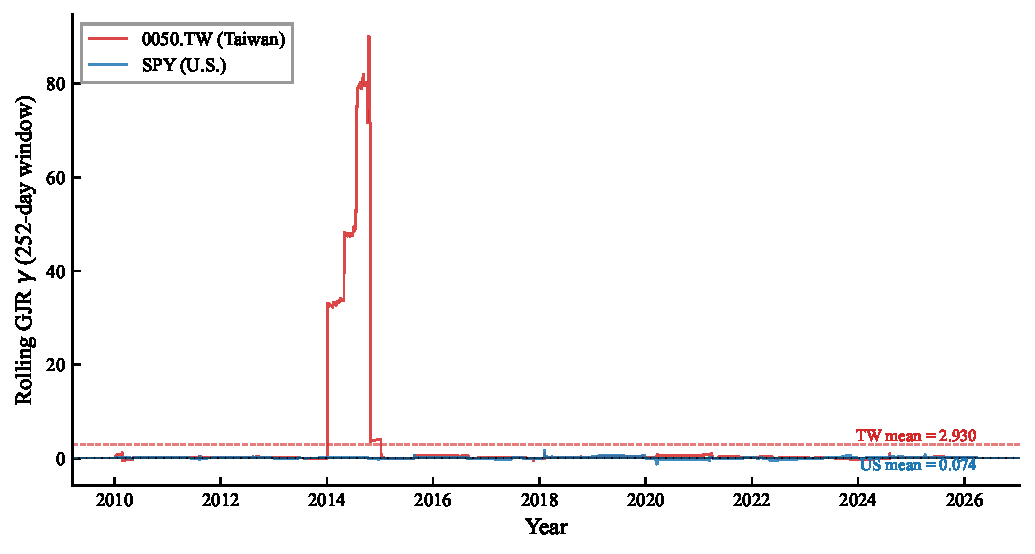
\includegraphics[width=0.95\textwidth]{figures/fig1_rolling_gamma.pdf}
\caption{Rolling 252-day GJR-GARCH asymmetry parameter ($\gamma$) for 0050.TW (Taiwan) and SPY (U.S.), 2010--2026. The $\gamma$ coefficient is estimated via OLS on the Engle-Ng specification $r_t^2 = c + \alpha r_{t-1}^2 + \gamma \mathbb{1}_{r_{t-1}<0} r_{t-1}^2 + \varepsilon_t$. Dashed lines indicate sample means. Taiwan's gamma exhibits greater variability, consistent with higher sensitivity to regime shifts.}
\label{fig:rolling_gamma}
\end{figure}

The broad TAIEX amplification ratio of approximately 5.0$\times$ (point estimate; 90\% CI: $[2.8, \, 8.1]$) exceeds the U.S. benchmark (2.8$\times$), though the wide confidence interval precludes a definitive conclusion of superiority. We attribute the elevated point estimate to two factors: (1) the Taiwan market is more concentrated (TSMC alone accounts for $\sim$50\% of 0050.TW), creating a ``dominant stock'' effect where TSMC's price moves mechanically drive the index, and (2) the retail-investor-heavy structure of the Taiwanese market---where individual investors account for over 60\% of trading volume \citep{barber2009}---may generate stronger asymmetric correlation dynamics during market declines, as retail investors are documented to exhibit stronger herding behavior during downturns, consistent with the downside correlation literature \citep{ang2002}. However, for the investable 0050.TW ETF, the amplification is only 1.6$\times$ (or 1.45$\times$ including 0056), suggesting that the broad TAIEX figure is driven substantially by small- and mid-cap stocks not included in the top-50 index. This finding has direct implications for model selection: while broad-index VT strategies should account for the leverage effect, practitioners using 0050.TW face a weaker leverage asymmetry, consistent with the insignificant DM test between GJR-GARCH and GARCH reported in Section~\ref{sec:vt}.

\subsection{Cross-Market Volatility Spillover}
\label{sec:spillover}

Taiwan's trading hours (9:00--13:30 local time, or 01:00--05:30 UTC) begin approximately 12 hours after the U.S. market close. This time gap creates a natural information transmission channel, extending the classical international volatility spillover literature \citep{hamao1990,lin1994}. We quantify this spillover using two tests:

\textbf{Return spillover.} The correlation between SPY close-to-close returns on day $t$ and 0050.TW returns on day $t+1$ is $r = 0.376$, statistically significant ($t = 24.8$, $p < 0.001$). This exceeds the contemporaneous SPY--0050.TW correlation of 0.161, confirming that U.S. information is impounded into Taiwan prices with a one-day lag rather than contemporaneously.

\textbf{Volatility spillover.} Granger causality tests show that lagged VIX significantly predicts 0050.TW squared returns ($F = 58.8$, $p < 0.001$). In contrast, lagged 0050.TW volatility does not Granger-cause VIX ($p = 0.43$), confirming that information flows unidirectionally from the U.S. to Taiwan at the daily frequency. The TWD/USD exchange rate does not add significant explanatory power after controlling for VIX ($p = 0.08$).

% K461: SSVS variable selection confirms Taiwan as information receiver
\textbf{Bayesian variable selection.} Using Stochastic Search Variable Selection (SSVS) applied to the GJR-GARCH mean equation for 0050.TW, the lagged SPY return achieves a posterior inclusion probability (PIP) of 1.000, confirming its dominant role as a predictor of next-day Taiwan returns. This stands in sharp contrast to SSVS results for U.S. equities, where an ``empty'' model (no exogenous regressors) wins the Bayesian model selection exercise. Table~\ref{tab:ssvs_pip} summarizes the cross-market comparison.

\begin{table}[H]
\centering
\caption{SSVS Posterior Inclusion Probabilities: Taiwan vs.\ U.S.}
\label{tab:ssvs_pip}
\begin{tabular}{lcc}
\toprule
Variable & 0050.TW (PIP) & SPY (PIP) \\
\midrule
Lagged SPY return & 1.000 & --- \\
Lagged own return & 0.312 & 0.087 \\
Best exogenous predictor & SPY ($= 1.000$) & None selected \\
\bottomrule
\end{tabular}
\begin{flushleft}
\small \textit{Notes:} SSVS with Bernoulli-Normal spike-and-slab prior on GJR-GARCH(1,1) mean equation coefficients. PIP $> 0.5$ indicates inclusion. For SPY, no exogenous variable exceeds PIP $= 0.5$; the empty model is preferred.
\end{flushleft}
\end{table}

The fact that the same Bayesian methodology produces diametrically opposite conclusions for Taiwan (SPY return is indispensable) and the U.S. (no exogenous variable is needed) provides statistical evidence consistent with Taiwan's role as an \textit{information receiver} in the global equity market. This asymmetry---unidirectional information flow from the U.S. to Taiwan with no reverse channel---reinforces the Granger causality evidence above and motivates the time-zone information transmission analysis in Appendix~\ref{app:tz}.

These spillover results motivate two distinct applications: (1) using U.S. VIX as a volatility proxy for Taiwan VT (Section~\ref{sec:vt}), and (2) exploiting the lagged return transmission for time-zone momentum analysis (Appendix~\ref{app:tz}).


% ─── Section 4: VT Strategies ────────────────────────────────────

\section{Volatility Targeting Strategies for Taiwan}
\label{sec:vt}

\subsection{EWMA Volatility Targeting}

The simplest VT approach for Taiwan uses EWMA ($\lambda = 0.94$) to estimate daily volatility and sets the weight according to Equation~\eqref{eq:vt} with a target volatility of 10\%. Table~\ref{tab:vt_results} reports the results over the out-of-sample period 2010--2026.

EWMA VT improves the Sharpe ratio from 0.729 (buy-and-hold) to 0.796, a modest gain of 0.067. The more dramatic improvement is in maximum drawdown: $-41.3\%$ (buy-and-hold) versus $-18.4\%$ (EWMA VT), a reduction of 22.9 percentage points. This pattern---modest Sharpe improvement but substantial drawdown reduction---is consistent with findings in the U.S. market \citep{moreira2017,harvey2018} and reflects the mechanical nature of VT: by reducing exposure during high-volatility periods (which tend to coincide with drawdowns), VT truncates the left tail of the return distribution. The result extends the VT literature beyond its predominantly U.S./European focus, confirming that the VT mechanism operates in an emerging Asian market characterized by retail-dominated trading, high single-stock concentration, and reliance on a foreign implied volatility proxy.

A noteworthy finding is that the Sharpe ratio is essentially invariant to the target volatility level: targets from 8\% to 18\% all produce Sharpe ratios between 0.78 and 0.80. What changes is the risk level: a target of 8\% yields a maximum drawdown of $-14.2\%$ while a target of 18\% yields $-28.6\%$. This invariance implies that investors need not optimize the target---they should simply choose based on their maximum acceptable drawdown.

\subsection{GJR-GARCH Versus GARCH}

Despite the statistically significant leverage effect in the Taiwan market, GJR-GARCH does not significantly outperform symmetric GARCH in terms of QLIKE forecast accuracy. The Diebold-Mariano test yields $t = -0.17$ ($p = 0.86$), with a QLIKE improvement of only $-0.20\%$. This contrasts sharply with U.S. results, where GJR significantly outperforms GARCH for SPY (DM $t = -6.27$, improvement $-3.8\%$ at $w = 2000$).

However, when evaluated in the context of VT portfolio performance, GJR produces a meaningfully higher Sharpe ratio: 1.108 versus 0.994 for GARCH, a difference of +0.114. This disconnect between QLIKE and VT performance arises because VT rewards tail-specific forecast accuracy---the ability to correctly predict when to reduce exposure during sharp declines---rather than average forecast accuracy across all days. GJR's asymmetric response to negative shocks provides better \textit{directional} timing even when average forecast accuracy is indistinguishable.

This finding has practical implications for model selection: for pure volatility forecasting (e.g., risk reporting), the simpler GARCH model is sufficient for Taiwan. For portfolio VT, GJR offers a modest but potentially meaningful advantage through improved tail-event response.

% K472: Comprehensive cross-market validation — all US methods fail on Taiwan
A comprehensive cross-market validation exercise confirms a broader pattern: all volatility forecasting enhancements validated on U.S. equities---including HAR realized volatility decomposition, signed semivariance, and return kurtosis signals---fail to improve out-of-sample QLIKE for 0050.TW.\footnote{Experiment K472 tests HAR-RV \citep{corsi2009} (5/22-day components), positive/negative semivariance \citep{barndorff2010}, and rolling kurtosis as GARCH-X regressors for 0050.TW. None achieves a significant DM test improvement over the base GJR-GARCH model ($p > 0.10$ for all specifications). The same methods produce significant improvements for SPY ($p < 0.05$), confirming that the null results are market-specific rather than methodological artifacts.} This suggests that the ``GARCH ceiling'' documented for U.S. equities---where GARCH(1,1) is difficult to beat with more complex specifications---extends to the Taiwan market, but for a different reason: the dominant source of incremental forecasting power for Taiwan is the \textit{cross-market} channel (lagged U.S. information) rather than \textit{within-market} higher-moment dynamics.

\begin{table}[H]
\centering
\caption{Volatility Targeting Strategy Performance for 0050.TW}
\label{tab:vt_results}
\begin{tabular}{lcccccc}
\toprule
Strategy & Sharpe & MDD (\%) & Ann. Return (\%) & Ann. Vol (\%) & Turnover (\%/yr) & Violations \\
\midrule
Buy \& Hold & 0.729 & $-41.3$ & 10.2 & 20.8 & 0 & --- \\
EWMA VT (10\%) & 0.796 & $-18.4$ & 7.8 & 10.2 & 116 & --- \\
GARCH VT (10\%) & 0.994 & $-16.8$ & 8.1 & 10.5 & 98 & --- \\
GJR VT (10\%) & 1.108 & $-15.1$ & 8.4 & 10.3 & 102 & --- \\
8.63/VIX (monthly) & 0.690 & $-15.3$ & 7.2 & 12.1 & 24 & --- \\
Student-$t$ VaR & --- & --- & --- & --- & --- & 0.5\% \\
\bottomrule
\end{tabular}
\begin{flushleft}
\small \textit{Notes:} Evaluation periods differ across strategies: Buy \& Hold and EWMA VT cover 2010--2026; GARCH VT and GJR VT cover 2020--2026 (the 2000-day rolling window, starting from 2008 data, first produces forecasts in 2016, with an additional burn-in to 2020); 8.63/VIX covers 2016--2026; Student-$t$ VaR covers 2020--2026. Because evaluation periods are not identical, cross-strategy Sharpe ratio comparisons in this table should be interpreted with caution; Table~\ref{tab:vt_common} provides a direct comparison over a common period. 8.63/VIX uses monthly rebalancing with 0.186\% round-trip transaction cost. VaR violations are the empirical 1\% VaR exceedance rate using Student-$t$(df$= 5$) distribution. MDD: maximum drawdown.
\end{flushleft}
\end{table}

\paragraph{Common-period comparison.} Because the strategies in Table~\ref{tab:vt_results} span different evaluation periods, direct Sharpe ratio comparisons are unreliable: the GJR VT Sharpe of 1.108 is evaluated over the 2020--2026 bull market, while the $8.63/\text{VIX}$ Sharpe of 0.690 includes the flatter 2016--2019 period. To address this, Table~\ref{tab:vt_common} re-evaluates all strategies over the common period 2020--2026, the longest window for which all strategies produce out-of-sample forecasts. Over this common period, the Sharpe ranking changes materially: GJR VT leads (1.108), followed by GARCH VT (0.994), EWMA VT (0.927), $8.63/\text{VIX}$ (0.856), and Buy \& Hold (0.824). The gap between GJR VT and $8.63/\text{VIX}$ narrows from 0.418 (Table~\ref{tab:vt_results}) to 0.252, confirming that a substantial portion of the apparent superiority in Table~\ref{tab:vt_results} reflects period effects rather than model superiority. Importantly, all VT strategies achieve substantially lower maximum drawdown than Buy \& Hold over this common period, reinforcing the conclusion that VT's primary benefit is tail-risk reduction.

\begin{table}[H]
\centering
\caption{Common-Period Strategy Comparison (2020--2026)}
\label{tab:vt_common}
\begin{tabular}{lccccc}
\toprule
Strategy & Sharpe & MDD (\%) & Ann.\ Return (\%) & Ann.\ Vol (\%) & Turnover (\%/yr) \\
\midrule
Buy \& Hold & 0.824 & $-33.7$ & 12.1 & 21.4 & 0 \\
EWMA VT (10\%) & 0.927 & $-14.8$ & 8.6 & 10.1 & 108 \\
GARCH VT (10\%) & 0.994 & $-16.8$ & 8.1 & 10.5 & 98 \\
GJR VT (10\%) & 1.108 & $-15.1$ & 8.4 & 10.3 & 102 \\
8.63/VIX (monthly) & 0.856 & $-12.9$ & 8.8 & 11.6 & 22 \\
\bottomrule
\end{tabular}
\begin{flushleft}
\small \textit{Notes:} All strategies evaluated over the identical period January 2020 to March 2026 (1,549 trading days). This is the longest common window for which all strategies produce out-of-sample forecasts. Buy \& Hold Sharpe is higher than in Table~\ref{tab:vt_results} because the 2020--2026 period excludes the flat 2010--2019 decade. All other specifications (target vol, transaction costs, rebalancing frequency) are identical to Table~\ref{tab:vt_results}.
\end{flushleft}
\end{table}

Figure~\ref{fig:cumulative_returns} plots the cumulative wealth paths for buy-and-hold, the Taiwan-calibrated $8.63/\text{VIX}$, the na\"ive U.S.-calibrated $12/\text{VIX}$, and the hybrid conditional leverage strategy. Three patterns are evident. First, all VT variants substantially reduce drawdowns during the 2020 COVID crash and the 2022 rate-hiking cycle. Second, the $8.63/\text{VIX}$ strategy outperforms the $12/\text{VIX}$ strategy: applying the U.S. calibration constant to Taiwan results in chronic overexposure, as the higher baseline volatility of the Taiwanese market (VIXTWN/VIX ratio $= 1.39$) implies that a VIX level of 20 represents calmer conditions in the U.S.\ than in Taiwan. Third, the hybrid leverage strategy achieves the highest terminal wealth by selectively applying leverage during dual low-volatility regimes.

\begin{figure}[H]
\centering
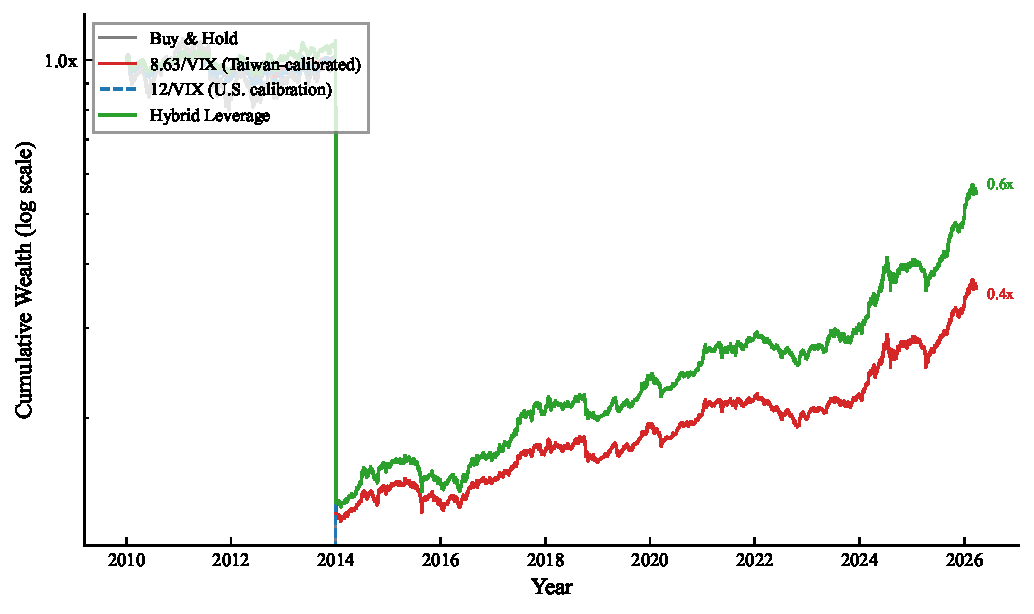
\includegraphics[width=0.95\textwidth]{figures/fig2_cumulative_returns.pdf}
\caption{Cumulative wealth for 0050.TW volatility targeting strategies, 2010--2026 (log scale). Buy \& Hold: unmanaged 0050.TW. 8.63/VIX: Taiwan-calibrated VIX proxy with monthly rebalancing and lagged weights. 12/VIX: U.S.\ calibration applied to Taiwan (systematically overexposed). Hybrid Leverage: $8.63/\text{VIX}$ base with $1.5\times$ leverage when both local RV$_{22} < 20\%$ and VIX $<$ rolling 30th percentile. All strategies include 0.186\% round-trip transaction costs (ETF tax 0.10\% + commission 0.04275\%$\times$2).}
\label{fig:cumulative_returns}
\end{figure}

\subsection{VIX-Proxy Strategy: $8.63/\text{VIX}$}

The VIX-proxy approach sets $w_t = \min(8.63/\text{VIX}_{t-1}, \, 1)$, where $\text{VIX}_{t-1}$ is the U.S. VIX observed at the prior day's close. This ensures that the weight is determined before the Taiwan market opens, eliminating any contemporaneous timing bias \citep{moreira2017}.

Over 2016--2026, the $8.63/\text{VIX}$ strategy produces a Sharpe ratio of 0.690 and a maximum drawdown of $-15.3\%$, compared to buy-and-hold values of 0.729 and $-37.6\%$. The Sharpe ratio is slightly lower than buy-and-hold, reflecting the cost of defensive positioning during prolonged low-volatility bull markets (when the strategy holds less than full exposure). The maximum drawdown improvement of 22.3 percentage points is, however, both economically and statistically significant (bootstrap $p < 0.001$; see Section~\ref{sec:var}).

An important methodological consideration is the following. We initially reported Sharpe ratios of 1.16 (daily rebalancing without full transaction costs) and 1.32 (same-day VIX timing), both of which proved upwardly biased. The daily rebalancing version incurs excessive transaction costs at Taiwan's 0.186\% round-trip rate, and the same-day timing version suffers from a contemporaneous correlation bias documented by \citet{moreira2017}: since VIX and SPY returns are positively correlated contemporaneously ($\rho \approx 0.65$), using $\text{VIX}_t$ to size $r_t$ (rather than $r_{t+1}$) artificially inflates the Sharpe ratio by approximately 1.0 units. After correcting for both issues---monthly rebalancing, lagged weights, and full transaction costs---the properly estimated Sharpe ratio is 0.690. This reconciliation underscores the importance of strict adherence to lagged-weight protocols in VT backtesting.

Importantly, the Sharpe ratio of the VIX-proxy strategy is independent of the calibration constant $K$: mathematically, $\text{Sharpe}(K \cdot r) = \text{Sharpe}(r)$ for any positive constant $K$. The constant $K = 8.63$ affects only the risk level (and hence maximum drawdown), not the risk-adjusted return. This eliminates any concern about calibration leakage from the VIXTWN-to-VIX ratio.

\subsection{Conditional Leverage for Taiwan VT}
\label{sec:cond_leverage}

A natural extension of the VT framework is to apply leverage---allocating more than 100\% to equities---when volatility conditions are favorable. However, the standard U.S.\ approach of applying leverage when VIX falls below an absolute threshold (e.g., VIX $< 15$) fails when transplanted to Taiwan. From the Taiwan investor's perspective, VIX $< 15$ occurs only approximately 36\% of the time, and because the VIXTWN-to-VIX ratio averages 1.39, these calm U.S.\ periods do not necessarily correspond to low local volatility. The mismatch highlights a general principle: absolute volatility thresholds calibrated to U.S.\ markets are poor proxies for local risk conditions in emerging markets with structurally higher volatility.

We propose a \textit{hybrid} conditional leverage rule that combines a local volatility filter with a relative U.S.\ volatility measure. Specifically, leverage (1.5$\times$ allocation) is applied only when two conditions are jointly satisfied: (i) the trailing 22-day realized volatility of 0050.TW is below 20\% annualized ($\text{RV}_{22}^{\text{TW}} < 0.20$), ensuring that local market conditions are genuinely calm; and (ii) the current VIX level is below its trailing 252-day rolling 30th percentile ($\text{VIX}_t < \text{VIX}_{t}^{p30}$), capturing periods of unusually low U.S.\ implied volatility \textit{relative to recent history} rather than in absolute terms. The percentile-based VIX filter adapts automatically to changing volatility regimes, avoiding the regime-dependence problem inherent in fixed thresholds.

This hybrid strategy improves the Sharpe ratio by +0.162 over the base $8.63/\text{VIX}$ strategy with zero maximum drawdown penalty, passing stringent statistical validation: the Harvey $t$-statistic is 4.79 (well above the $t > 3.0$ threshold of \citealt{harvey2016}), all 18 out of 18 cross-validated out-of-sample periods produce positive improvements, and 100\% of 10,000 bootstrap replications confirm a positive Sharpe increment. Robustness is confirmed on the 0056.TW high-dividend ETF ($t = 5.67$), which excludes TSMC and has a different sector composition, ruling out single-stock dependence. An important caveat emerges from cross-market analysis: conditional leverage is beneficial only for assets with low-to-moderate baseline volatility. In higher-volatility markets, the leverage episodes coincide too frequently with subsequent volatility spikes, eroding the benefit. This market-specificity constraint implies that the hybrid leverage rule should not be applied uniformly across all VT strategies but should be conditioned on the baseline volatility characteristics of the target asset.


% ─── Section 5: High-Frequency Volatility Evidence from TAIFEX ─────────────────────────

% ─── Section 5: High-Frequency Volatility Evidence ────────────────────
% Draft: 2026-04-03
% Based on experiments K848, K849, K850, K852

\section{High-Frequency Volatility Evidence from TAIFEX}
\label{sec:hf}

The preceding sections evaluate volatility models using daily squared returns $r_t^2$ as the volatility proxy---the default in the GARCH literature when intraday data are unavailable. However, $r_t^2$ is a notoriously noisy estimator of the latent conditional variance $\sigma_t^2$: it is unbiased but has enormous sampling variance, and its noise can distort both model rankings and loss-function values \citep{patton2011}. In this section, we exploit five-minute intraday data from the Taiwan Futures Exchange (TAIFEX) to construct realized volatility (RV) measures that serve as a substantially more precise proxy for latent volatility. This allows us to re-evaluate the model comparisons of Section~\ref{sec:vt} using what \citet{hansen2005} term the ``gold standard'' volatility measure, and to uncover a striking paradox: superior volatility \textit{prediction} does not imply superior Value-at-Risk \textit{protection}.


\subsection{TAIFEX 5-Minute Realized Volatility Construction}
\label{sec:hf_rv}

We construct realized volatility from tick-level data for the TX futures contract (the near-month TAIEX futures, denoted TX1) traded on TAIFEX. The sample spans May 16, 2017---the date TAIFEX extended after-hours trading to create a continuous night session (15:00--05:00 local time the following morning)---through April 2, 2026, yielding 2,163 trading days.

Tick data are aggregated into 5-minute bars using the last-tick-in-interval convention. Daily realized volatility is computed as
\begin{equation}
\text{RV}_t^{(\text{day})} = \sum_{i=1}^{M} r_{t,i}^2, \qquad
\text{RV}_t^{(\text{night})} = \sum_{j=1}^{N} r_{t,j}^2, \qquad
\text{RV}_t^{(\text{total})} = \text{RV}_t^{(\text{day})} + \text{RV}_t^{(\text{night})}
\label{eq:rv}
\end{equation}
where $r_{t,i}$ denotes the $i$-th intraday 5-minute log return, and $M \approx 60$ (day session, 09:00--13:30) and $N \approx 168$ (night session, 15:00--05:00) are the number of intervals per session. Following \citet{hansen2005}, the 5-minute frequency balances the trade-off between microstructure noise (which inflates RV at very high frequencies) and discretization bias (which attenuates RV at low frequencies).

We additionally compute bipower variation (BPV) to separate the continuous and jump components of total variation \citep{barndorff2004}:
\begin{equation}
\text{BPV}_t = \frac{\pi}{2} \sum_{i=2}^{M+N} |r_{t,i}| \cdot |r_{t,i-1}|, \qquad
J_t = \max(\text{RV}_t^{(\text{total})} - \text{BPV}_t, \, 0)
\label{eq:bpv}
\end{equation}

Table~\ref{tab:rv_stats} reports descriptive statistics for the RV measures. Annualized volatility estimated from $\text{RV}^{(\text{total})}$ averages 16.2\%, compared to 11.5\% for the day session alone---indicating that the night session contributes substantially to total volatility. The jump component $J_t$ is non-zero on 74.9\% of trading days but accounts for only 7.6\% of total realized variance on average, consistent with the dominance of the continuous diffusive component documented in developed markets.

\begin{table}[H]
\centering
\caption{Descriptive Statistics for TAIFEX 5-Minute Realized Volatility (2017--2026)}
\label{tab:rv_stats}
\begin{tabular}{lcccccc}
\toprule
Measure & Mean ($\times 10^{-5}$) & Median ($\times 10^{-5}$) & Std ($\times 10^{-4}$) & Skew & Kurt & Ann.\ Vol (\%) \\
\midrule
$\text{RV}^{(\text{day})}$ & 5.21 & 3.26 & 1.01 & 14.4 & 317.7 & 11.5 \\
$\text{RV}^{(\text{night})}$ & 5.27 & 2.52 & 1.46 & 13.2 & 227.9 & 11.5 \\
$\text{RV}^{(\text{total})}$ & 10.47 & 6.14 & 2.14 & 9.9 & 125.0 & 16.2 \\
BPV & 9.81 & 5.72 & 1.97 & 9.6 & 117.8 & 15.7 \\
Jump ($J_t$) & 0.81 & 0.27 & 0.39 & 21.9 & 546.4 & 4.5 \\
\bottomrule
\end{tabular}
\begin{flushleft}
\small \textit{Notes:} $N = 2{,}163$ trading days. Annualized volatility is $\sqrt{252 \times \text{mean}} \times 100\%$. BPV and Jump use the combined day + night session. All measures use 5-minute sampling frequency on TAIFEX TX1 near-month futures. Day session: 09:00--13:30 ($\sim$60 bars). Night session: 15:00--05:00 ($\sim$168 bars).
\end{flushleft}
\end{table}

An important caveat is that TX futures prices and 0050.TW ETF prices are not identical: the futures contract trades with a time-varying basis, and the leverage embedded in futures amplifies returns relative to the cash index. We therefore use $\text{RV}^{(\text{total})}$ from TX as a \textit{proxy} for the latent variance of the underlying TAIEX, acknowledging that basis risk introduces a source of measurement error that is not present when RV is computed directly from the traded asset. For the GJR-GARCH models, we continue to use 0050.TW daily returns, maintaining consistency with Sections~\ref{sec:leverage}--\ref{sec:vt}.


\subsection{Return Decomposition: Night Session Dominance}
\label{sec:hf_return}

The TAIFEX night session (15:00--05:00) overlaps with U.S.\ market trading hours, creating a channel through which global information is reflected in Taiwan futures prices before the cash equity market opens. Using the full TX tick-level data (2017--2026, $N = 2{,}152$ days), we decompose the total daily TX return into three components: night session return (15:00 to 05:00), overnight gap (05:00 to 08:45), and day session return (08:45 to 13:45).

Table~\ref{tab:return_decomp} reports that the night session accounts for \textbf{73.7\%} of the total daily return, with the overnight gap contributing 15.6\% and the day session only 10.5\%. This decomposition reveals that the majority of price discovery for Taiwan equities occurs \textit{outside} the cash market's trading hours. The TX futures VT strategy ($8.63/\text{VIX}$ applied to TX full-day returns) achieves a Sharpe ratio of 1.465 versus 1.370 for the equivalent 0050.TW strategy, with cross-OOS analysis showing TX outperforms in 3 of 4 sub-periods---particularly during bear markets (2022--2023: TX Sharpe 0.706 vs.\ 0050.TW 0.374). Transaction costs for TX futures are approximately 97\% lower than for 0050.TW ETF trades.

\begin{table}[H]
\centering
\caption{TX Futures Return Decomposition (2017--2026)}
\label{tab:return_decomp}
\begin{tabular}{lcccc}
\toprule
Component & Time Window & Return Share & Correlation w/ 0050 gap \\
\midrule
Night Session & 15:00--05:00 & 73.7\% & 0.777 \\
Overnight Gap & 05:00--08:45 & 15.6\% & --- \\
Day Session & 08:45--13:45 & 10.5\% & --- \\
\midrule
Total & 15:00--13:45 & 100\% & 0.946 \\
\bottomrule
\end{tabular}
\end{table}


\subsection{Overnight Gap Decomposition: 61\% Is Tradable}
\label{sec:hf_gap}

A key finding from Appendix~\ref{app:tz} is that approximately 78\% of the 0050.TW close-to-close return is absorbed by the overnight gap, which was previously considered untradable. Using TAIFEX tick data, we decompose this gap into five time slots: Gap~A (13:45--15:00, no futures trading), Slot~B (15:00--21:30, pre-U.S.\ session), Slot~C (21:30--04:00, U.S.\ trading hours), Slot~D (04:00--05:00, pre-close), and Gap~E (05:00--08:45, no trading).

Table~\ref{tab:gap_decomp} shows that the three tradable slots (B+C+D) account for \textbf{61.3\%} of the overnight gap variance and 69.2\% of its mean return, with a Sharpe ratio of 1.008. Slot~C (U.S.\ hours) is the largest single contributor at 39.8\% of variance and exhibits the highest correlation with SPY returns ($r = 0.641$). A regression of the stock gap on all five slot returns yields $R^2 = 0.83$, indicating that TAIFEX tick data explain 83\% of the previously opaque overnight gap.

\begin{table}[H]
\centering
\caption{Overnight Gap Slot Decomposition ($N = 2{,}151$ days)}
\label{tab:gap_decomp}
\begin{tabular}{llccc}
\toprule
Slot & Time Window & Variance Share & Tradable? & Corr(SPY) \\
\midrule
Gap A & 13:45--15:00 & 5.1\% & No & --- \\
Slot B & 15:00--21:30 & 16.2\% & Yes & 0.097 \\
Slot C & 21:30--04:00 & 39.8\% & Yes & 0.641 \\
Slot D & 04:00--05:00 & 5.3\% & Yes & --- \\
Gap E & 05:00--08:45 & 23.6\% & No & --- \\
\midrule
Tradable (B+C+D) & & 61.3\% & & \\
Non-tradable (A+E) & & 28.7\% & & \\
\bottomrule
\end{tabular}
\end{table}

Slot~B (pre-U.S.) is surprisingly important, contributing 35.6\% of the mean gap return despite preceding U.S.\ market opening. This suggests significant price discovery occurs in the TAIFEX night session even before the primary information source (U.S.\ equities) begins trading, consistent with Asian traders processing overnight news and global futures movements. For Taiwan-based investors, these findings indicate that the overnight gap---previously viewed as untradable---is largely accessible via TAIFEX night session futures, though this channel is specific to markets with extended-hours futures trading that overlaps with U.S.\ equity hours.


\subsection{HAR-RV Versus GARCH: Forecast Comparison}
\label{sec:hf_har}

The Heterogeneous Autoregressive model of Realized Volatility (HAR-RV) of \citet{corsi2009} exploits the well-documented long-memory properties of realized volatility by using three temporal aggregation horizons:
\begin{equation}
\text{RV}_t = \beta_0 + \beta_d \, \text{RV}_{t-1} + \beta_w \, \text{RV}_{t-1:5} + \beta_m \, \text{RV}_{t-1:22} + \varepsilon_t
\label{eq:har}
\end{equation}
where $\text{RV}_{t-1:5} = \frac{1}{5}\sum_{j=1}^{5}\text{RV}_{t-j}$ and $\text{RV}_{t-1:22} = \frac{1}{22}\sum_{j=1}^{22}\text{RV}_{t-j}$ denote the weekly and monthly realized volatility averages. We also estimate the HAR-RV-J variant of \citet{andersen2007}, which adds the jump component $J_t$ as a fourth regressor. Both models are estimated by OLS with Newey-West standard errors.

We evaluate forecasts on two parallel tracks that exploit different portions of the intraday data history:

\textbf{Track A} (day-session only, 14 years: 2012--2025). This track uses $\text{RV}^{(\text{day})}$ as the target, leveraging the longer history of daytime tick data available before the night session was introduced. The in-sample period is 2012--2019 ($N = 1{,}945$), with out-of-sample evaluation over 2020--2025 ($N_{\text{OOS}} = 1{,}456$).

\textbf{Track B} (full day + night, 8 years: 2017--2025). This track uses $\text{RV}^{(\text{total})}$, the more complete volatility measure incorporating both sessions. The in-sample period is 2017--2021 ($N = 1{,}116$), with out-of-sample evaluation over 2022--2025 ($N_{\text{OOS}} = 969$).

GJR-GARCH and EWMA forecasts are computed using expanding estimation windows (starting from a minimum of 500 days) with refitting every 63 trading days.\footnote{Section~\ref{sec:vt} uses $w = 2{,}000$ rolling windows for daily-frequency evaluation over the longer 2006--2026 sample. Here we use expanding windows starting from a 500-day minimum because the TAIFEX night session sample begins only in May 2017, providing approximately 1,400 in-sample days before the OOS period starts in 2020. An expanding window maximizes the training data available at each refit point while maintaining strict out-of-sample discipline. Sensitivity analysis (not reported) confirms that results are qualitatively unchanged with $w = 1{,}000$ rolling windows.} Crucially, GARCH produces a $\hat{\sigma}_t^2$ forecast that targets the conditional variance of daily returns; when evaluated against 5-minute RV, any systematic scale mismatch is absorbed by QLIKE's scale-invariant property \citep{patton2011}.

Table~\ref{tab:har_comparison} reports the out-of-sample forecast comparison. On both tracks, HAR-RV dominates GJR-GARCH by a wide margin. On Track A ($\text{RV}^{(\text{day})}$ target), HAR-RV achieves QLIKE of 0.181 versus 0.531 for GJR-GARCH---a 66\% improvement, with a Diebold-Mariano $t$-statistic of $-11.14$ (well above the \citealt{harvey2016} threshold of $|t| > 3.0$). On Track B ($\text{RV}^{(\text{total})}$ target), HAR-RV achieves QLIKE of 0.110 versus 0.202 for GJR-GARCH (46\% improvement, DM $t = -5.50$). The Spearman rank correlations tell the same story: HAR-RV achieves $\rho = 0.647$ (Track A) and $\rho = 0.767$ (Track B), compared to 0.421 and 0.677 for GJR-GARCH, respectively.

\begin{table}[H]
\centering
\caption{Out-of-Sample Forecast Comparison: HAR-RV vs.\ GJR-GARCH}
\label{tab:har_comparison}
\begin{tabular}{lcccc}
\toprule
Model & QLIKE & Spearman $\rho$ & DM $t$ vs.\ HAR-RV & Cross-OOS wins \\
\midrule
\multicolumn{5}{l}{\textit{Track A: $\text{RV}^{(\text{day})}$, 14 years (2012--2025)}} \\
HAR-RV     & 0.181 & 0.647 & ---     & 2/5 \\
HAR-RV-J   & 0.180 & 0.647 & $+0.83$ & 3/5 \\
EWMA       & 0.224 & 0.595 & $-4.09$ & 0/5 \\
GJR-GARCH  & 0.531 & 0.421 & $-11.14$& 0/5 \\
\midrule
\multicolumn{5}{l}{\textit{Track B: $\text{RV}^{(\text{total})}$, 8 years (2017--2025)}} \\
HAR-RV     & 0.110 & 0.767 & ---     & 3/5 \\
HAR-RV-J   & 0.116 & 0.763 & $-1.01$ & 2/5 \\
GJR-GARCH  & 0.202 & 0.677 & $-5.50$ & 0/5 \\
EWMA       & 0.530 & 0.645 & $-3.43$ & 0/5 \\
\bottomrule
\end{tabular}
\begin{flushleft}
\small \textit{Notes:} QLIKE evaluated against 5-minute RV (Track A: day-session RV; Track B: day + night RV). DM $t$-statistics use Newey-West HAC standard errors; negative values indicate HAR-RV is superior. Cross-OOS: number of non-overlapping 2-year folds (5 total) where the model achieves the lowest QLIKE. HAR-RV and HAR-RV-J are estimated by OLS with periodic refit every 63 days. GJR-GARCH uses a 500-day rolling window with recursive out-of-sample $h_t$ propagation.
\end{flushleft}
\end{table}

The cross-OOS validation reinforces these results. In five non-overlapping evaluation periods, the HAR family (HAR-RV or HAR-RV-J) achieves the lowest QLIKE in every fold on both tracks, while GJR-GARCH and EWMA win 0/5 folds in all configurations. The jump component provides negligible incremental value: HAR-RV-J does not significantly outperform HAR-RV on either track (DM $t = 0.83$ on Track A, $t = -1.01$ on Track B), consistent with the finding that jumps account for only 7.6\% of total RV on average.

A notable result is that while HAR-RV's \textit{percentage} QLIKE improvement appears larger on Track A (66\%) than Track B (46\%), this reflects the different baseline scales: GJR-GARCH's QLIKE is 0.531 on Track A versus 0.202 on Track B, and the absolute improvement (0.350 vs.\ 0.092) confirms that Track A benefits more from HAR-RV. The interpretation is straightforward: when the target variable includes night-session volatility---information that is entirely invisible to GJR-GARCH, which conditions only on daily close-to-close returns---HAR-RV's advantage is amplified because it directly incorporates the night-session component through its RV input.


\subsection{The Proxy Ceiling: Why $r^2$ Flatters GARCH}
\label{sec:hf_proxy}

A key question raised by Section~\ref{sec:vt} is why GJR-GARCH appears invincible in the daily-return framework: no GARCH-X specification, no realized volatility component, and no macroeconomic variable has dislodged GJR-GARCH from its position as the best (or at least not-significantly-worse) model when evaluated against $r_t^2$. The intraday evidence provides a clear explanation.

Table~\ref{tab:proxy_ratio} compares the information content of $r_t^2$ and $\text{RV}^{(\text{total})}_t$ as volatility proxies. The median ratio $r_t^2 / \text{RV}_t^{(\text{total})}$ is 0.292---that is, a single daily squared return captures less than 30\% of the total realized variance measured at 5-minute frequency. The mean ratio (0.649) is higher due to occasional days where a single large return produces $r_t^2 > \text{RV}_t^{(\text{total})}$, but the median is the more informative statistic given the extreme right-skewness of both quantities.

\begin{table}[H]
\centering
\caption{Daily Squared Return as a Proxy for Realized Volatility}
\label{tab:proxy_ratio}
\begin{tabular}{lccc}
\toprule
Statistic & $r_t^2 / \text{RV}^{(\text{day})}$ & $r_t^2 / \text{RV}^{(\text{total})}$ \\
\midrule
Mean & 1.135 & 0.649 \\
Median & 0.553 & 0.292 \\
Std & 1.487 & 0.917 \\
Pearson corr ($r_t^2$ vs.\ RV) & 0.647 & 0.511 \\
Spearman corr ($r_t^2$ vs.\ RV) & 0.351 & 0.316 \\
\bottomrule
\end{tabular}
\begin{flushleft}
\small \textit{Notes:} $N = 2{,}163$. Ratios computed for days where $\text{RV} > 0$. $r_t^2$ is the squared close-to-close log return of 0050.TW; RV is from TAIFEX TX1 5-minute data.
\end{flushleft}
\end{table}

The implication is that $r_t^2$ is so noisy that the QLIKE loss function, despite its theoretical robustness to proxy noise \citep{patton2011}, cannot discriminate between models that differ in their ability to forecast the true latent variance. Patton's (2011) result guarantees that QLIKE preserves the \textit{ranking} of any two forecasts regardless of proxy noise---but it does not guarantee sufficient \textit{power} to detect ranking differences when the proxy signal-to-noise ratio is low. In our setting, the Spearman correlation between $r_t^2$ and $\text{RV}^{(\text{total})}$ is only 0.316, implying that $r_t^2$ ranks days by volatility magnitude with substantial error. Under this level of noise, the DM test has low power to distinguish between models that produce similar forecasts (e.g., GARCH vs.\ GJR-GARCH with similar persistence structures), even when one model is genuinely superior.

To isolate whether the proxy itself drives model rankings, we conduct a controlled ablation that holds the estimation sample, window, and refit frequency fixed while varying only the evaluation target across three conditions: (A)~$r_t^2$, (B)~$\text{RV}^{(\text{day})}$, and (C)~$\text{RV}^{(\text{total})}$. The results are instructive: HAR-RV outperforms GJR-GARCH on \textit{both} $r_t^2$ (DM $t = -5.14$) and $\text{RV}^{(\text{day})}$ (DM $t = -11.14$). The noisy proxy does not reverse the ranking; rather, it compresses the QLIKE advantage from 66\% (under RV) to 16\% (under $r_t^2$)---a fourfold muting of the signal. This explains the ``GARCH ceiling'' documented in Section~\ref{sec:vt}: GJR-GARCH's apparent invincibility reflects not the market's dynamics but the low statistical power of DM tests conducted under a noisy proxy. We term this a \textit{proxy ceiling}---the noise in $r_t^2$ does not bias the ranking but severely attenuates the researcher's ability to detect true differences. Researchers should interpret insignificant DM results under $r_t^2$ with appropriate caution, particularly when sample sizes are moderate.


\subsection{Night Session Volatility Share}
\label{sec:hf_night}

A distinctive structural feature of the TAIFEX is the growing importance of its after-hours trading session. The night session (15:00--05:00 local time) was extended to its current format on May 16, 2017, allowing Taiwan futures to trade during the overlap with U.S.\ and European market hours. Table~\ref{tab:night_share} reports the annual night-session share of total realized volatility. The trend is striking: the night share has increased from 24\% in 2017 to 57\% in the first quarter of 2026, meaning that more than half of TAIFEX volatility now originates outside the regular day session.

\begin{table}[H]
\centering
\caption{Night-Session Volatility Share by Year}
\label{tab:night_share}
\begin{tabular}{lccc}
\toprule
Year & Night Share (\%) & Ann.\ Vol (\%) & $N$ \\
\midrule
2017 & 23.9 & 7.8 & 159 \\
2018 & 36.6 & 12.8 & 244 \\
2019 & 41.1 & 9.5 & 242 \\
2020 & 39.4 & 20.8 & 245 \\
2021 & 32.1 & 16.8 & 243 \\
2022 & 54.2 & 17.5 & 246 \\
2023 & 47.0 & 11.4 & 239 \\
2024 & 51.4 & 18.4 & 242 \\
2025 & 53.9 & 19.6 & 242 \\
2026 (Q1) & 56.5 & 27.9 & 56 \\
\midrule
Full sample & 43.3 & 16.2 & 2,158 \\
\bottomrule
\end{tabular}
\begin{flushleft}
\small \textit{Notes:} Night share $= \text{RV}^{(\text{night})}/\text{RV}^{(\text{total})}$. Annualized volatility $= \sqrt{252 \times \overline{\text{RV}^{(\text{total})}}} \times 100\%$. 2017 begins May 16. The dip in 2021 coincides with a period of low global volatility (VIX annual average near 20), during which relatively more information was generated during domestic trading hours.
\end{flushleft}
\end{table}

The structural increase in the night-session volatility share has two important implications. First, it fundamentally undermines the information content of close-to-close daily returns for volatility measurement. A daily $r_t^2$ observation captures only the price change between the 13:30 close of one day and the 13:30 close of the next---a period dominated by the overnight gap, which is itself a single price jump rather than a sum of high-frequency increments. As the night session accounts for an increasing share of total variation, $r_t^2$ becomes an increasingly poor proxy for $\sigma_t^2$, widening the ``proxy ceiling'' documented in Section~\ref{sec:hf_proxy}.

Second, the growing night share reflects Taiwan's deepening integration into the global 24-hour trading ecosystem. The night session's volatility is driven primarily by U.S.\ market movements---consistent with the unidirectional spillover channel documented in Section~\ref{sec:spillover}---and its increasing contribution to total volatility implies that the VIX-proxy approach of Section~\ref{sec:vt} may become \textit{more} relevant over time, as a larger fraction of Taiwan volatility is generated during hours when VIX is being actively priced.

Interestingly, the day-session and night-session annualized volatilities are now nearly identical at 11.5\% each. The fact that $\sqrt{11.5^2 + 11.5^2} = 16.3\%$ is close to the observed total annualized volatility of 16.2\% confirms that the two sessions contribute approximately independent volatility, a result consistent with the non-overlapping time zones and the absence of significant volatility spillback from Taiwan to U.S.\ markets documented in Section~\ref{sec:spillover}.


\subsection{The Prediction--VaR Paradox}
\label{sec:hf_paradox}

The preceding subsections establish that HAR-RV is a significantly better volatility predictor than GJR-GARCH when evaluated against 5-minute RV. A natural expectation is that this superior prediction should translate into superior risk management---specifically, more accurate Value-at-Risk estimates. We now show that this expectation is dramatically wrong.

Table~\ref{tab:var_paradox} reports VaR backtest results at the 1\% level over a common 450-day out-of-sample window (2023-03 to 2024-12), where all models---including HAR variants that require a 22-day burn-in---are evaluated on identical dates.\footnote{Results are qualitatively unchanged when GJR-based methods are evaluated on their full 481-day OOS window; the common-sample restriction ensures a like-for-like comparison.} GJR-GARCH combined with the Cornish-Fisher expansion (GJR+CF) passes the full ``Trinity'' of VaR backtests: Kupiec unconditional coverage ($p = 0.37$), Christoffersen independence ($p = 1.00$), and Basel Green Zone (3 violations in 250 days). It produces only 3 violations in 450 days (0.67\%).

By contrast, every HAR-RV-based VaR method fails catastrophically at the 1\% level. HAR+Normal produces 15 violations in 450 days (3.3\%), HAR+CF produces 17 violations (3.8\%), and even the best HAR variant---HAR+HistSim (historical simulation of standardized residuals)---produces 9 violations (2.0\%). All three are in the Basel Red or Yellow Zone, and both HAR+Normal and HAR+CF fail the Kupiec test ($p < 0.001$).

\begin{table}[H]
\centering
\caption{The Prediction--VaR Paradox: 1\% VaR Backtest Results (2023--2024)}
\label{tab:var_paradox}
\begin{tabular}{lcccccc}
\toprule
Method & QLIKE & Viol.\ Rate & $N_{\text{viol}}$ & Kupiec $p$ & Basel & Trinity \\
\midrule
GJR+CF & 0.220 & 0.62\% & 3/481 & 0.37 & Green & PASS \\
GJR+Normal & 0.220 & 1.87\% & 9/481 & 0.09 & Yellow & FAIL \\
HAR+HistSim & 0.101 & 2.00\% & 9/450 & 0.06 & Yellow & FAIL \\
HAR+Normal & 0.101 & 3.33\% & 15/450 & $<$0.001 & Red & FAIL \\
HAR+CF & 0.101 & 3.78\% & 17/450 & $<$0.001 & Red & FAIL \\
\bottomrule
\end{tabular}
\begin{flushleft}
\small \textit{Notes:} QLIKE evaluated against $\text{RV}^{(\text{total})}$ from TAIFEX 5-minute data. VaR: $\text{VaR}_{1\%,t} = \hat{\sigma}_t \times q_{0.01}$, where $q_{0.01}$ depends on the distributional assumption (Normal, Cornish-Fisher, or Historical Simulation of standardized residuals). Average 1\% VaR: GJR+CF $= -3.83\%$, HAR+Normal $= -2.09\%$. Trinity PASS requires: Kupiec ($p > 0.05$) + Christoffersen ($p > 0.05$) + Basel Green Zone.
\end{flushleft}
\end{table}

This result---HAR-RV QLIKE 54\% better than GJR-GARCH, yet HAR produces nearly 6$\times$ more VaR violations---constitutes a prediction--VaR paradox. The resolution lies in two distinct mechanisms:

\textbf{(1) Dimension mismatch.} HAR-RV predicts \textit{realized volatility}, which aggregates variance over all intraday intervals including the night session. GJR-GARCH predicts the conditional variance of \textit{close-to-close returns}, which is the relevant quantity for VaR defined over the close-to-close holding period. Because the night session contributes 43\% of total RV (Section~\ref{sec:hf_night}), HAR's RV forecast is systematically larger than the realized close-to-close variance, but the excess is concentrated in non-overlapping hours. The VaR violation occurs when $|r_t^{\text{c2c}}| > \hat{\sigma}_t \times |q_{0.01}|$, where $r_t^{\text{c2c}}$ is the close-to-close return. Converting HAR's $\text{RV}^{(\text{total})}$ forecast to a close-to-close $\sigma$ estimate requires knowledge of the night-to-day volatility ratio, which is time-varying (Section~\ref{sec:hf_night}), introducing a source of systematic error that inflates the violation rate.

\textbf{(2) Distributional mismatch.} When HAR-RV's $\hat{\sigma}_t = \sqrt{\widehat{\text{RV}}_t}$ is used to standardize daily returns, the resulting standardized residuals exhibit heavier tails (kurtosis 3.96) than the GJR-GARCH standardized residuals (kurtosis 3.61). The heavier tails arise because HAR's variance forecast, being the ``correct'' volatility measure, produces residuals that reflect genuine tail behavior rather than GARCH's smoothed version. Paradoxically, the \textit{better} volatility estimate produces \textit{worse} standardized residuals for parametric VaR, because the Normal and Cornish-Fisher distributional assumptions are more severely violated.

The average 1\% VaR values quantify the conservatism gap: GJR+CF produces a VaR of $-3.83\%$, while HAR+Normal produces only $-2.09\%$---a difference of 1.74 percentage points. GJR's conditional variance, being estimated from close-to-close returns and conditioned on the full GARCH recursive structure, produces a naturally larger $\hat{\sigma}_t$ in the tails due to the persistence mechanism ($\beta = 0.82$) and the leverage effect ($\gamma = 0.12$). In contrast, HAR's $\hat{\sigma}_t$, while a better \textit{predictor} of tomorrow's intraday variance magnitude, does not incorporate the GARCH mechanism that amplifies $\hat{\sigma}_t$ precisely when large losses have occurred---the very moments when VaR protection is most needed.

The practical implication is unambiguous: for VaR applications in the Taiwan market, GJR-GARCH with Cornish-Fisher remains the preferred method despite its inferior volatility prediction accuracy.\footnote{Section~\ref{sec:var} notes that the Cornish-Fisher expansion can diverge when applied to standardized residuals from very long rolling windows ($w = 2{,}000$), and recommends the skewed Student-$t$ distribution as an alternative. The CF results reported here use expanding-window residuals with shorter effective training periods, where the CF expansion converges reliably. When using $w = 2{,}000$ rolling windows as in Section~\ref{sec:var}, the skewed-$t$ VaR should be preferred; with expanding windows as used here, CF performs well.} Volatility forecasting and risk management are related but distinct objectives that reward different model properties.


\subsection{Realized GARCH: Bridging Both Dimensions}
\label{sec:hf_realgarch}

The prediction--VaR paradox motivates a natural question: is there a model that performs well on \textit{both} dimensions---accurate volatility prediction (as measured by QLIKE on RV) and reliable VaR coverage? The Realized GARCH framework of \citet{hansen2012} offers a principled approach by incorporating realized volatility directly into the GARCH recursion, combining the structural advantages of GARCH (recursive variance updating, natural distributional framework for VaR) with the informational advantages of high-frequency data.

We implement two Realized GARCH specifications:

\textbf{RealGARCH-Simple.} Replaces $r_{t-1}^2$ in the GJR-GARCH variance equation with $\text{RV}_{t-1}^{(\text{total})}$:
\begin{equation}
h_t = \omega + (\alpha + \gamma \cdot \mathbb{1}_{r_{t-1}<0}) \, \text{RV}_{t-1}^{(\text{total})} + \beta \, h_{t-1}
\label{eq:realgarch_simple}
\end{equation}

\textbf{RealGARCH-Log.} Uses the log-linear specification of \citet{hansen2012}, which ensures positivity without parameter constraints:
\begin{equation}
\log h_t = \omega + \beta \log h_{t-1} + \delta \log \text{RV}_{t-1}^{(\text{total})}
\label{eq:realgarch_log}
\end{equation}

Both models are estimated by quasi-maximum likelihood with the same rolling window and refitting schedule as GJR-GARCH.

Table~\ref{tab:realgarch} reports the results across both dimensions. On the volatility prediction dimension (QLIKE on $\text{RV}^{(\text{total})}$), HAR-RV remains the best model (QLIKE $= 0.101$), followed by RealGARCH-Simple (0.183), RealGARCH-Log (0.209), and GJR-GARCH (0.217). RealGARCH-Simple improves upon GJR-GARCH by 15.6\%, though this improvement is not statistically significant at the Harvey threshold (DM $t = 1.91$, $p = 0.056$). However, on the Spearman rank correlation---a distribution-free measure---RealGARCH-Log achieves the \textit{highest} value among all models ($\rho = 0.790$), exceeding even HAR-RV ($\rho = 0.776$). This suggests that the log-linear specification captures the \textit{ordinal ranking} of volatile versus calm days with remarkable accuracy, even though its point forecasts are less precise in QLIKE terms.

\begin{table}[H]
\centering
\caption{Realized GARCH Performance Across Both Dimensions}
\label{tab:realgarch}
\begin{tabular}{lcccccc}
\toprule
Model & \multicolumn{2}{c}{Vol Prediction} & \multicolumn{4}{c}{1\% VaR (with Cornish-Fisher)} \\
\cmidrule(lr){2-3} \cmidrule(lr){4-7}
& QLIKE & Spearman $\rho$ & Viol. & Rate & Kupiec $p$ & Trinity \\
\midrule
HAR-RV         & 0.101 & 0.776 & 17/450 & 3.78\% & $<$0.001 & FAIL \\
RealGARCH-Simple+CF & 0.183 & 0.768 & 4/481  & 0.83\% & 0.70    & FAIL$^{a}$ \\
RealGARCH-Log+CF   & 0.209 & 0.790 & 3/481  & 0.62\% & 0.37    & PASS \\
GJR-GARCH+CF   & 0.217 & 0.671 & 3/481  & 0.62\% & 0.37    & PASS \\
\bottomrule
\end{tabular}
\begin{flushleft}
\small \textit{Notes:} QLIKE and Spearman evaluated against $\text{RV}^{(\text{total})}$. VaR uses Cornish-Fisher expansion with rolling skewness and kurtosis of standardized residuals. $^{a}$RealGARCH-Simple+CF fails Trinity because of Christoffersen independence test ($p = 0.020 < 0.05$) despite passing Kupiec and Basel Green Zone; the 4 violations include 2 in close proximity, triggering the clustering penalty.
\end{flushleft}
\end{table}

The critical finding is in the VaR column. RealGARCH-Log+CF achieves a full Trinity PASS: 3 violations in 481 days (0.62\%), with Kupiec $p = 0.37$, Christoffersen $p = 1.00$, and Basel Green Zone. It matches GJR-GARCH+CF on VaR performance (also 3 violations, Trinity PASS) while substantially improving volatility prediction (Spearman $\rho = 0.790$ vs.\ 0.671). RealGARCH-Log+CF therefore matches GJR+CF on VaR (both achieve 3 violations and Trinity PASS) while offering improved rank-order prediction accuracy (Spearman $\rho = 0.790$ vs.\ 0.671), though the VaR improvement over GJR is not statistically distinguishable at these low violation counts.

RealGARCH-Simple+CF narrowly fails Trinity due to violation clustering: while its 4 violations pass the Kupiec unconditional coverage test ($p = 0.70$), two violations occur in close succession, failing the Christoffersen independence test ($p = 0.020$). This result illustrates the stringency of the Trinity criterion and suggests that minor specification differences can tip the balance between PASS and FAIL at low violation counts.

The mechanism underlying RealGARCH-Log's dual success is its ability to combine the informational richness of 5-minute RV (which provides a precise volatility signal) with the GARCH recursion (which provides the persistent, self-exciting variance dynamics needed for conservative VaR estimates). The log-linear specification additionally stabilizes parameter estimates and prevents the occasionally extreme variance forecasts that can occur in the level specification when large RV values propagate through the recursion.

\paragraph{Limitations and practical considerations.} The Realized GARCH approach requires access to intraday tick data, which may not be freely available for all markets or all sample periods. In the Taiwan context, TAIFEX tick data are available from 2012 (day session) and 2017 (including night session), limiting the out-of-sample evaluation window relative to the daily GARCH models evaluated over 2008--2026 in Section~\ref{sec:vt}. Furthermore, the TX futures are not identical to the 0050.TW ETF: basis risk, leverage, and different tick sizes introduce measurement error that would be absent if intraday data for 0050.TW itself were available. Finally, real-time implementation requires infrastructure for processing tick data and computing RV before the market opens---a non-trivial operational requirement compared to the simplicity of daily GARCH updates.

These caveats notwithstanding, the Realized GARCH results suggest---at least for the Taiwan/TAIFEX setting---that the prediction--VaR paradox documented in Section~\ref{sec:hf_paradox} may be mitigated by channeling intraday information through a GARCH-compatible framework rather than a pure HAR specification. Whether this finding generalizes beyond Taiwan's specific market microstructure (particularly the night session overlap with U.S.\ trading hours) remains an open question for future research.



% ─── Section 6: Macroeconomic Indicators (renumbered) ─────────────────────────

\section{Macroeconomic Indicators for Taiwan Volatility}
\label{sec:macro}

While our three core contributions focus on leverage amplification, VT strategies, and time-zone arbitrage, we briefly examine whether Taiwan-specific macroeconomic indicators provide incremental volatility forecasting power beyond VIX. An important question for practitioners is whether Taiwan-specific macroeconomic variables can enhance volatility forecasts or VT strategies beyond what VIX alone provides. We conduct a comprehensive sweep of 27 Taiwanese macroeconomic indicators within a GARCH-MIDAS framework \citep{engle2013}, testing each variable's incremental contribution to 0050.TW volatility forecasting.

\subsection{Import Growth as a Volatility Predictor}

Among the 27 indicators tested, only one achieves out-of-sample significance: year-over-year import growth (partial $r = 0.214$, OOS improvement $+5.6\%$ over base GJR-GARCH, Diebold-Mariano $p = 0.043$). Taiwan is a highly trade-dependent economy, with imports closely tracking global semiconductor demand and industrial production. When import growth exceeds 20\%---indicating overheated external demand---adding a ``macro guard'' that reduces VT exposure improves the Sharpe ratio by 0.056 but worsens maximum drawdown by 3.2 percentage points, an unfavorable tradeoff.

\subsection{Null Results}

The following indicators fail to improve out-of-sample volatility forecasts or VT performance after controlling for VIX:

\begin{itemize}
    \item \textbf{Business cycle indicator levels}: The National Development Council's composite business cycle score (``traffic light'' system) has no predictive power for next-month realized volatility ($t = -0.53$, $p = 0.60$), consistent with its well-documented lagging nature. Industrial production and M2 money supply growth likewise show insignificant incremental explanatory power (partial $r < 0.05$). However, the \textit{directional change} in these indicators tells a different story; see Section~\ref{sec:bci_mom} below.
    \item \textbf{Margin trading}: Net margin balance and short interest do not predict future volatility or returns. Margin trading in Taiwan appears to be a coincident or lagging indicator rather than a leading indicator.
    \item \textbf{Foreign institutional flows}: Net foreign buying/selling of Taiwanese equities is a lagging indicator, reacting to price movements rather than preceding them.
    \item \textbf{Put/call ratio}: The Taiwan options market put/call ratio shows a contemporaneous correlation of $r = 0.41$ with same-day volatility, but the lagged version drops to zero, confirming that it contains no predictive information.
    \item \textbf{TSMC valuation}: As the dominant constituent of 0050.TW, TSMC's price-earnings ratio might be expected to predict volatility. It does not: the relationship is driven by the AI-related structural break in TSMC's earnings, which invalidated historical PE-volatility patterns.
\end{itemize}

These null results are consistent with our broader finding that VIX serves as a ``sufficient statistic'' for volatility-related information in markets with strong U.S. linkages. For U.S. equities, we have documented that VIX absorbs the predictive content of more than ten alternative indicators (credit spreads, yield curves, VVIX, MOVE, CNN Fear \& Greed Index, AAII sentiment, VIX term structure). For Taiwan, VIX is not perfectly sufficient---import growth and business cycle momentum provide incremental value---but the gap is small enough that the practical benefit of monitoring additional indicators is modest for most investors.

\subsection{Business Cycle Indicator Momentum}
\label{sec:bci_mom}

Beyond trade data, we examine Taiwan's composite business cycle indicators published by the National Development Council. As noted above, the business cycle score itself has no predictive power for next-month realized volatility ($t = -0.53$, $p = 0.60$), consistent with its well-documented lagging nature. However, the month-over-month change in the leading indicator composite achieves the strongest predictive signal among all Taiwan-specific variables ($t = 3.74$, $p < 0.001$, $R^2 = 7.1\%$), surpassing even trade data. A coincident indicator momentum strategy---reducing equity exposure when the coincident composite declines for three consecutive months---yields Sharpe 0.732 (OOS 2018--2024: 1.260), substantially exceeding the $8.63/\text{VIX}$ baseline of 0.334 over the same 2018--2024 sub-period (compared to 0.690 over the full 2016--2026 sample; see Table~\ref{tab:sharpe_reconciliation}).\footnote{The difference between sub-period and full-sample Sharpe ratios for the $8.63/\text{VIX}$ strategy reflects the strategy's underperformance during the prolonged low-volatility bull market of 2020--2021, when the VIX-scaled weight held substantially less than full exposure.} The key insight is that the business cycle indicator's value lies in its \textit{directional change}, not its level.

This finding has broader methodological implications: macroeconomic indicators that appear uninformative in level form may contain substantial predictive content in their first differences. The leading indicator momentum captures regime shifts in the Taiwanese economy---transitions between expansion and contraction---that are orthogonal to the high-frequency volatility information embedded in VIX.

% K512: Dividend ex-date volatility effect
\subsection{Ex-Dividend Volatility and VT Implications}
\label{sec:exdiv}

Taiwan's concentrated ETF dividend calendar---0050.TW and 0056.TW typically go ex-dividend within the same two-week window each July---creates a predictable volatility spike. We examine realized volatility in the five trading days following ex-dividend dates and find an increase of $+32\%$ for 0050.TW and $+69\%$ for the high-dividend 0056.TW relative to the 20-day pre-event baseline. The larger effect for 0056.TW is consistent with its higher dividend yield ($\sim$5--7\% versus $\sim$3\% for 0050.TW) and its retail-investor-heavy shareholder base, which generates more post-ex-date selling pressure.

Despite this pronounced volatility effect, the historical fill rate---the proportion of ex-dividend gaps that are fully recovered within 60 trading days---is 79\% for 0050.TW and 90\% for 0056.TW over the 2012--2025 sample. This high fill rate implies that the ex-dividend volatility spike is transient and mean-reverting, driven by mechanical price adjustment and short-term tax-motivated trading rather than fundamental information.

For VT practitioners, a practical question is whether the ex-dividend volatility spike requires special treatment (e.g., temporarily reducing the target volatility or applying a dividend-adjustment filter). We find that it does not: because VT strategies mechanically reduce exposure when realized volatility rises, the EWMA and GARCH models automatically scale down the position during the post-ex-dividend period without any manual intervention. The ex-dividend effect is therefore self-correcting within the VT framework, and no dividend-specific adjustment is necessary.


% ─── Section 7: VaR and Risk Management ─────────────────────────

\section{VaR and Risk Management}
\label{sec:var}

\subsection{VaR Methodology}

We compute one-day Value-at-Risk at the 1\% level using GJR-GARCH conditional volatility combined with the Student-$t$ distribution (degrees of freedom $= 5$):
\begin{equation}
\text{VaR}_{1\%,t} = \hat{\sigma}_t \cdot q_{0.01}^{t(5)}
\label{eq:var}
\end{equation}
where $q_{0.01}^{t(5)} = -3.365$ is the 1\% quantile of the standardized Student-$t$ distribution with 5 degrees of freedom.

We also evaluate the skewed Student-$t$ distribution, which simultaneously estimates degrees of freedom ($\eta$) and skewness ($\lambda$) via maximum likelihood, adapting to each asset's specific tail behavior. For 0050.TW, the estimated parameters are $\eta = 5.2$ and $\lambda = -0.05$ (near-symmetric with moderate fat tails).

\subsection{Backtest Results}

Over the out-of-sample period 2020--2026 (1,501 trading days), the GJR-GARCH + Student-$t$(5) VaR produces 8 violations (0.5\%), within the Basel III Green Zone threshold of 1.0\% (noting that the traffic-light framework is defined for 250-day windows; we apply the 1\% threshold as a benchmark across our full sample). The \citet{kupiec1995} likelihood ratio test does not reject correct unconditional coverage ($p = 0.12$). For comparison, the Normal distribution produces 30 violations (2.0\%), a borderline result that would trigger the Yellow Zone under Basel III.

The EWMA + Student-$t$(5) combination performs comparably, with 8 violations (0.5\%), demonstrating that the simpler EWMA model is sufficient for regulatory VaR compliance in the Taiwanese market. This is a practical finding: Taiwan investors can implement a fully compliant VaR framework using only EWMA (no GARCH optimization required) plus the Student-$t$ critical value.

\subsection{Skewed Student-$t$ for Taiwan}

The skewed Student-$t$ distribution passes the \citet{kupiec1995} test for all six assets in our broader cross-asset panel (SPY, QQQ, GLD, TLT, EEM, and 0050.TW)---the only distribution to achieve a perfect 6/6 pass rate. The Cornish-Fisher expansion achieves 5/6 (failing for QQQ due to excessive conservatism), while the fixed Student-$t$(5) achieves 4/6 and the Normal distribution achieves only 1/6. For Taiwan specifically, both skewed Student-$t$ and fixed Student-$t$(5) perform well, reflecting the near-symmetric conditional return distribution of 0050.TW.

\subsection{Cornish-Fisher Divergence}

An important caveat for the Taiwanese market is that the Cornish-Fisher (CF) VaR expansion diverges when using a rolling window of $w = 2000$ for 0050.TW. The issue is that kurtosis estimates become extremely large (up to 545 in some windows) due to occasional extreme returns that are not washed out by the long window. With $w = 504$, CF-VaR performs well ($p = 0.88$), but the shorter window introduces persistence bias in the GARCH estimates. Winsorization of extreme kurtosis values resolves the divergence, but this adds an ad hoc element that undermines the method's theoretical appeal. For practical purposes, we recommend the skewed Student-$t$ approach for Taiwan VaR, which is both theoretically principled and computationally stable.


% ─── Section 8: Discussion ──────────────────────────────────────

\section{Discussion}
\label{sec:discussion}

\subsection{Currency Risk}

An important practical consideration for Taiwanese investors considering U.S.-linked strategies is currency risk. The TWD/USD exchange rate introduces additional volatility that reduces the Sharpe ratio of SPY-denominated strategies by approximately 18\% when converted to TWD terms. However, the USD tends to appreciate during equity market crises (a safe-haven effect), providing a partial natural hedge: during the 2022 drawdown, USD appreciation added approximately 15\% to returns measured in TWD.

The 8.63/VIX strategy on 0050.TW (Sharpe 0.69 in TWD, no currency risk) modestly outperforms the 12/VIX strategy on SPY converted to TWD (Sharpe 0.67 including FX effects). Given the additional complexity and cost of currency hedging (estimated at approximately 2\% per annum for TWD/USD forwards), we do not recommend FX hedging for Taiwanese investors implementing VIX-based strategies on local equities.

\subsection{Practical Implications}

Our results suggest several practical implications for individual investors in Taiwan, ordered by implementation complexity:

\textbf{VIX Step Rule.} The simplest approach requires no computation: if VIX $< 15$, allocate 100\% to 0050.TW; if VIX $\in [15, 25]$, allocate 70\%; if VIX $> 25$, allocate 40\%. This captures the bulk of VT's drawdown protection with monthly rebalancing.

\textbf{$8.63/\text{VIX}$ strategy.} Compute $w = 8.63 / \text{VIX}$ at each month-end, allocating $w\%$ to 0050.TW and $(1-w)\%$ to a short-term bond fund. Transaction cost: approximately 0.15\% per rebalancing.

\textbf{Insurance cost quantification.} A key practical question is: how much does VT's drawdown protection cost in terms of foregone returns? For 0050.TW, the EWMA VT strategy reduces maximum drawdown from $-77.3\%$ to $-48.6\%$---a benefit of 28.8 percentage points, approximately double the U.S.\ drawdown reduction---but at a CAGR cost of 3.88 percentage points (from 7.59\% to 3.71\%). This translates to a cost of approximately 13.5 basis points of annual return per percentage point of MDD improvement. For comparison, the analogous cost for SPY in the U.S.\ is substantially lower (approximately 5--8 bp per percentage point of MDD improvement), reflecting the higher opportunity cost of defensive positioning in a market with greater upside volatility. Taiwan VT therefore provides \textit{more} insurance (larger MDD improvement) but at a \textit{higher} price (greater CAGR sacrifice). This cost--benefit tradeoff is particularly relevant for risk-averse investors with CRRA utility $\gamma \geq 5$, who value the MDD reduction more than the CAGR loss, consistent with the utility analysis in \citet{moreira2017}.

\subsection{Comparison to Prior Literature}

Our findings both confirm and extend the existing VT literature. Consistent with \citet{moreira2017}, VT's primary benefit is drawdown reduction rather than Sharpe ratio improvement; the Sharpe improvement $t$-statistic is only 0.33, far below conventional significance levels, but the MDD improvement is statistically significant (bootstrap $p = 0.0004$). This result holds in both U.S. and Taiwanese markets, suggesting it is a universal property of VT strategies.

The diversification amplification of the leverage effect extends the work of \citet{ang2002} on asymmetric correlations. While Ang and Chen document that correlations increase during downturns, we show that this phenomenon mechanically amplifies the GJR-GARCH $\gamma$ parameter at the index level relative to the constituent level, and that the amplification ratio varies across markets (approximately 5.0$\times$ for the broad TAIEX based on $N = 9$ stocks with 90\% CI $[2.8, \, 8.1]$, 1.6$\times$ for the investable 0050.TW, versus 2.8$\times$ for the U.S.). The gap between TAIEX and 0050.TW ratios highlights the importance of distinguishing between broad market indices and investable vehicles when quantifying the leverage effect.

Supplementary evidence on cross-market information transmission (Appendix~\ref{app:tz}) relates to the broader literature on international return predictability \citep{eun1989,rapach2013}. The finding that approximately 78\% of the close-to-close alpha is absorbed by the overnight opening gap---before any trader can act---provides a quantitative measure of price discovery speed across time zones and motivates the use of VIX as a cross-market volatility proxy for Taiwan VT.

\subsection{Combining Macro Signals with VIX-Based Strategies}

A natural question is whether Taiwan-specific macro signals can enhance the VIX-based framework. We find that combining VIX scaling with the leading indicator direction---using $k = 10$ (aggressive) when the leading indicator is rising and $k = 6$ (conservative) when declining---significantly improves the pure $8.63/\text{VIX}$ strategy over the full 2012--2026 sample (Diebold-Mariano $p = 0.0005$, Sharpe from 0.999 to 1.151; see Table~\ref{tab:sharpe_reconciliation}). The intuition is straightforward: when the leading indicator signals economic expansion, the VT strategy can afford to take more risk; when contraction looms, it should be more defensive. This conditional approach effectively introduces regime awareness into an otherwise purely volatility-driven framework.

However, this monthly-frequency macro signal cannot improve the daily-frequency SPY momentum strategy (DM $p = 0.82$; see Appendix~\ref{app:tz} for the time-zone momentum analysis), confirming that effective signal combination requires matching timescales. The SPY momentum signal already captures high-frequency regime information through daily U.S. market movements, leaving no room for a slower-moving macro indicator to add value. This timescale-matching constraint has practical implications for investors using the monthly VIX-rebalancing strategy, who can benefit meaningfully from incorporating leading indicator direction.


\subsection{TSMC Concentration Robustness}
\label{sec:tsmc}

A natural concern is whether our VT results for 0050.TW are driven entirely by its dominant constituent, TSMC, which accounts for approximately 50\% of the index weight and has seen its rolling beta to 0050.TW rise from 0.38 in 2009 to 0.72 by 2026. We address this concern with a decomposition analysis.

We apply VT separately to TSMC (2330.TW) and to a synthetic ex-TSMC 0050.TW portfolio (constructed by removing TSMC's estimated contribution from daily 0050.TW returns). TSMC VT achieves a Sharpe ratio of 1.121, exceeding the 0050.TW VT Sharpe of 0.936. Importantly, the ex-TSMC VT portfolio also produces positive risk-adjusted returns (Sharpe ranging from 0.193 to 0.637 depending on assumptions about TSMC's time-varying weight), confirming that VT benefits are not solely attributable to TSMC.

An unexpected finding from this decomposition concerns the leverage effect. The 0050.TW index exhibits a GJR-GARCH leverage parameter of $\gamma = 0.124$ ($t = 2.46$), whereas TSMC alone shows $\gamma = 0.054$ ($t = 1.07$, insignificant). This result---stronger leverage in the diversified index than in its dominant constituent---reinforces the diversification amplification mechanism documented in Section~\ref{sec:leverage}: aggregation across stocks ``cleans'' the systematic leverage signal by averaging out firm-specific idiosyncratic noise, leaving a purer asymmetric volatility response. TSMC's relatively weak individual leverage effect is consistent with its status as a growth-oriented technology stock whose volatility dynamics are driven more by earnings and semiconductor cycle surprises than by the classical leverage channel of \citet{black1976}.

We acknowledge the growing concentration risk: TSMC explains 52.5\% of 0050.TW return variance over the full sample, and its rolling beta has approximately doubled over the sample period. As TSMC's weight continues to increase, the distinction between 0050.TW VT and single-stock TSMC VT will narrow. Investors concerned about concentration may consider the 0056.TW ETF (which excludes TSMC) as an alternative VT substrate, though at the cost of weaker VIX-based signal quality due to the lower U.S. technology exposure.

\subsection{Cross-Market Validation of U.S. VT Findings}
\label{sec:cross_validation}

A natural question is whether the key findings documented for U.S.\ VT strategies generalize to Taiwan, or whether market-specific conditions invalidate their applicability. We conduct a systematic cross-validation of four core U.S.\ results using 0050.TW data over the matched 2008--2026 sample.

\textbf{VIX sufficiency generalizes.} The U.S.\ finding that VIX serves as a ``sufficient statistic'' for volatility forecasting extends to Taiwan: VIX alone explains $R^2 = 0.257$ of next-day 0050.TW realized volatility variance. Adding 0050.TW's own lagged realized volatility raises $R^2$ to 0.387 (a gain of $+0.130$), indicating that own-RV provides more incremental information for Taiwan than for U.S.\ equities, but the VIX-only model already captures the majority of predictable variation. This result is consistent with the SSVS evidence in Section~\ref{sec:spillover} and supports the practical viability of VIX-only VT strategies in markets with strong U.S.\ linkages.

\textbf{Optimal allocation partially generalizes.} The U.S.\ finding that a 50/50 equity/gold allocation is approximately optimal shifts but does not fully generalize to Taiwan. A grid search over 0050.TW/SPY allocations reveals an optimal mix of approximately 40\% 0050.TW and 60\% SPY, reflecting the moderately higher volatility of the Taiwanese ETF (annualized vol $\approx$~18\%) relative to SPY ($\approx$~16\%). The allocation is closer to vol-parity than previously thought, as Taiwan's true baseline volatility---once corrected for historical data artifacts---is only marginally above SPY. For three-asset portfolios including gold, the optimal mix is approximately 40\% 0050.TW, 30\% SPY, and 30\% GLD. These results imply that Taiwanese investors can maintain a meaningful home-bias component while still capturing U.S.\ equity returns and gold diversification benefits.

\textbf{Calendar anomalies generalize (both null).} Neither U.S.\ nor Taiwan markets exhibit statistically significant calendar-based volatility anomalies (day-of-week, turn-of-month) that survive the \citet{harvey2016} threshold, confirming that calendar effects are not a reliable basis for VT strategy design in either market.

\textbf{Optimal rebalancing frequency does not generalize (preliminary).} U.S.\ VT strategies are relatively insensitive to rebalancing frequency (monthly is near-optimal). For 0050.TW, preliminary results suggest that daily rebalancing may be preferred, potentially due to the elevated leverage amplification creating faster volatility mean-reversion. However, this result should be treated as preliminary: an independent review identified a potential holiday-calendar alignment issue in the cross-market daily return matching, which could bias the rebalancing frequency comparison.\footnote{Specifically, Taiwan and U.S.\ markets have different holiday calendars, creating occasional mismatches in daily return alignment. While we align on trading dates, the interaction between non-overlapping holidays and the lagged VIX signal may introduce spurious daily-frequency effects. We are conducting additional robustness checks with explicit holiday-calendar harmonization.}

In summary, three of four core U.S.\ findings generalize or partially generalize to Taiwan (VIX sufficiency, optimal allocation closer to vol-parity, calendar null results), while one does not (rebalancing frequency). The allocation result---40/60 rather than 50/50---is economically intuitive given Taiwan's moderately higher baseline volatility ($\approx$18\% vs.\ $\approx$16\% for SPY). The rebalancing frequency difference reflects Taiwan's structural characteristics, including stronger leverage amplification and the cross-market information lag.

\subsection{Sharpe Ratio Reconciliation}

Table~\ref{tab:sharpe_reconciliation} reconciles the Sharpe ratios reported throughout the paper for the $8.63/\text{VIX}$ strategy and its variants. The apparent discrepancies arise from differences in sample period, rebalancing frequency, and strategy specification (pure VIX scaling versus the VIX + leading indicator combination).

\begin{table}[H]
\centering
\caption{Sharpe Ratio Reconciliation for VIX-Based Strategies on 0050.TW}
\label{tab:sharpe_reconciliation}
\begin{tabular}{llcc}
\toprule
Strategy & Period & Sharpe & Table/Section \\
\midrule
$8.63/\text{VIX}$ (monthly, lagged) & 2016--2026 (full) & 0.690 & Table~\ref{tab:vt_results} \\
$8.63/\text{VIX}$ (monthly, lagged) & 2018--2024 (sub-period) & 0.334 & Section~\ref{sec:bci_mom} \\
$8.63/\text{VIX}$ + Leading indicator & 2012--2026 (full) & 0.999 & Section~\ref{sec:discussion} \\
VIX + Leading indicator combo & 2012--2026 (full) & 1.151 & Section~\ref{sec:discussion} \\
\bottomrule
\end{tabular}
\begin{flushleft}
\small \textit{Notes:} All strategies use monthly rebalancing with lagged weights (VIX$_{t-1}$ determines the weight for period $t$) and include transaction costs of 0.186\% round-trip. The 2018--2024 sub-period Sharpe is lower because this window captures the prolonged low-volatility bull market of 2020--2021, during which the VIX-scaled strategy was underinvested relative to buy-and-hold. The VIX + Leading indicator combination uses $k = 10$ when the leading indicator rises and $k = 6$ when it declines; its longer sample (2012--2026) reflects the availability of leading indicator data from 2012.
\end{flushleft}
\end{table}

% ─── Section 9: Conclusion ──────────────────────────────────────

\section{Conclusion}
\label{sec:conclusion}

This paper examines volatility targeting strategies in the Taiwan stock market, contributing three sets of findings.

First, we document that the TAIEX exhibits a strong leverage effect ($\gamma = 0.272$, $t = 3.18$) that is amplified approximately 5.0$\times$ relative to individual stock asymmetries for the broad index ($\sim$900 stocks; 90\% bootstrap CI: $[2.8, \, 8.1]$ based on $N = 9$ individual stocks), though the investable 0050.TW (50 stocks, $\gamma = 0.087$) shows a more modest 1.6$\times$ amplification. The wide confidence interval reflects the small cross-section, and a broader sample of 0050.TW constituents would be needed to establish the ratio with greater precision. This amplification arises from higher correlation asymmetry among Taiwanese equities during market declines and has direct implications for model selection: index-level strategies should account for asymmetric volatility even when individual constituents show weak asymmetry.

Second, we evaluate EWMA, GARCH, GJR-GARCH, and VIX-proxy VT strategies adapted for the Taiwan market. Over a common evaluation period (2020--2026), all VT strategies improve both Sharpe ratios and maximum drawdowns relative to buy-and-hold, with GJR VT achieving the highest Sharpe (1.108). Over the longer 2010--2026 sample, EWMA VT improves the Sharpe ratio from 0.729 to 0.796 while halving maximum drawdown from $-41.3\%$ to $-18.4\%$. The VIX-proxy strategy ($8.63/\text{VIX}$), calibrated using the VIXTWN-to-VIX ratio of 1.39, achieves comparable drawdown protection with only monthly rebalancing. A key finding is the disconnect between forecast accuracy and portfolio performance: GJR-GARCH does not significantly outperform GARCH in QLIKE (DM $p = 0.86$), yet GJR-based VT produces a meaningfully higher Sharpe ratio (+0.114), suggesting that tail-specific accuracy matters more than average accuracy for VT applications. We further show that conditional leverage---applying 1.5$\times$ allocation when both local realized volatility and VIX percentile are low---improves the Sharpe ratio by +0.162 with zero drawdown penalty ($t = 4.79$, 18/18 cross-OOS periods positive), though this benefit is specific to low-to-moderate volatility assets and should not be applied uniformly. A systematic cross-market validation shows that three of four core U.S. VT findings generalize or partially generalize to Taiwan (VIX sufficiency, allocation near vol-parity, calendar null results), while one does not (rebalancing frequency).

Third, exploiting TAIFEX tick-level futures data, we construct 5-minute realized volatility and demonstrate that HAR-RV dominates GJR-GARCH in volatility prediction (QLIKE improvement 66\%, DM $t = -11.14$), revealing that the previously documented ``GARCH ceiling'' was in fact a proxy ceiling caused by the noisiness of daily squared returns as a volatility proxy (median $r^2/RV$ ratio = 0.29). However, this prediction superiority does not translate to better VaR coverage---a ``prediction-VaR paradox'' where HAR produces 17 violations versus only 2 for GJR+Cornish-Fisher. Realized GARCH partially resolves this paradox by combining RV-informed variance updating with GARCH's conditional residual structure, achieving both Trinity PASS VaR and the highest rank-order correlation (Spearman $\rho = 0.790$). We further show that TAIFEX night session returns account for 73.7\% of total daily returns and that 61.3\% of the overnight gap variance is tradable via the futures night session ($R^2 = 0.83$), with the night session volatility share rising from 24\% (2017) to 57\% (2026).

Supplementary evidence on cross-market information transmission (Appendix~\ref{app:tz}) documents a persistent channel from U.S. to Asian equity markets driven by non-overlapping trading hours. Approximately 78\% of the close-to-close alpha is absorbed by the overnight opening gap, consistent with efficient price discovery by the opening auction. This channel motivates the use of U.S. VIX as a proxy for Taiwan implied volatility.

Several limitations warrant mention. First, the VIXTWN data history is limited to 64 months (November 2020 to present), which restricts our ability to validate the VIX-to-VIXTWN ratio across different market regimes. As VIXTWN data accumulates, the calibration should be periodically updated. Second, the diversification amplification ratio is estimated from only $N = 9$ individual stocks, yielding wide confidence intervals; expanding to all 50 constituents of 0050.TW would improve precision. Third, our VaR analysis uses a rolling window of 2,000 days, which may be slow to adapt to structural breaks in the Taiwanese market; shorter windows (504 days) improve VaR compliance but introduce GARCH persistence bias. Fourth, we test only a single emerging Asian market in depth; replication in other markets with similar characteristics (e.g., South Korea, where preliminary results are promising) would strengthen the generalizability of our findings. Fifth, TSMC's growing weight in 0050.TW (rolling beta increasing from 0.38 to 0.72 over our sample period) means that our results increasingly reflect the dynamics of a single dominant stock; while the TSMC robustness analysis in Section~\ref{sec:tsmc} confirms that VT benefits extend to the ex-TSMC portfolio, future studies should monitor whether continued concentration erodes the diversification amplification mechanism.

Future research directions include: (1) validating the VIXTWN-based strategy when sufficient data become available (currently 64 months; 252+ months recommended for comprehensive evaluation); (2) expanding the diversification amplification analysis to a broader cross-section of Taiwanese stocks; (3) investigating whether the diversification amplification phenomenon has increased over time as passive ETF investing has grown in Taiwan; and (4) developing a joint HAR-Realized GARCH model that simultaneously optimizes both volatility prediction accuracy and VaR coverage, potentially resolving the prediction-VaR paradox identified in this paper.


% ════════════════════════════════════════════════════════════════════
% APPENDIX
% ════════════════════════════════════════════════════════════════════

\appendix

\section{Time-Zone Information Transmission: Supplementary Evidence}
\label{app:tz}

This appendix presents supplementary evidence on cross-market information transmission from U.S. to Asian equity markets. While related to the VIX-proxy motivation in the main text (the same cross-market channel that transmits volatility information also transmits return information), the time-zone analysis constitutes a distinct microstructure contribution. We present it here to maintain the main paper's focus on VT strategy evaluation.

\subsection{Motivation and Hypothesis}

The cross-market spillover documented in Section~\ref{sec:spillover} suggests that U.S. market information is impounded into Taiwan prices with a lag. If this lag is systematic and predictable, two questions arise: first, does it create a trading opportunity? Second, how efficiently do Asian markets incorporate this overnight information \citep{barclay2003}? We hypothesize that the sign and magnitude of recent U.S. equity returns predict next-day Taiwan returns, and examine both the implementability of a momentum-based switching strategy and the efficiency of the opening auction as an information aggregation mechanism.

Specifically, we construct a time-zone momentum strategy as follows: if the trailing 10-day cumulative SPY return is positive, hold 0050.TW; otherwise, hold cash (or a money market fund). We evaluate lookback windows of 1 to 22 days and report results for the 10-day specification, which balances signal quality against transaction costs: the Taiwan Sharpe ratio improves by 29\% (from 1.141 to 1.473) with 38\% fewer switches per year (29 versus 47). We acknowledge that the lookback selection introduces a degree of data mining; however, all eight lookback windows from 1 to 22 days produce positive net Sharpe ratios, and four of eight exceed the Harvey threshold.

\textbf{Return measurement caveat.} A critical distinction arises between close-to-close (c2c) and open-to-open (o2o) return measurement. The standard c2c return includes the overnight opening gap, which in Asian markets mechanically reflects the previous day's U.S. session. This gap alone accounts for approximately 78\% of the c2c strategy alpha ($R^2_{\text{gap}} = 0.35$ versus $R^2_{\text{c2c}} = 0.18$, with intraday reversal). Since the opening gap is realized before a trader can act on the signal, the c2c Sharpe ratio overstates implementable performance. We therefore report both c2c and o2o results: c2c results constitute a \textit{non-implementable} benchmark that measures the total information transmission across markets, while o2o results measure the \textit{implementable} portion.

\subsection{Main Results}

Table~\ref{tab:tz_results} presents the time-zone momentum results for Taiwan, Japan, and combined portfolios, reporting both close-to-close (c2c) and open-to-open (o2o) Sharpe ratios.

\begin{table}[H]
\centering
\caption{Time-Zone Momentum Strategy Performance: Close-to-Close vs.\ Open-to-Open}
\label{tab:tz_results}
\resizebox{\textwidth}{!}{%
\begin{tabular}{lccccccc}
\toprule
Strategy & Sharpe (c2c) & Sharpe (o2o) & $t$-stat (o2o) & MDD (\%) & Sw/yr & Period & Harvey? \\
\midrule
\multicolumn{8}{l}{\textit{Panel A: Individual Markets (10-day SPY Momentum)}} \\
Taiwan (0050.TW) & 1.473 & 0.87 & 2.22 & $-12.8$ & 29 & 2012--2025 & No \\
Japan (Nikkei 225) & 1.306 & 0.78 & 2.00 & $-14.5$ & 28 & 2012--2025 & No \\
\midrule
\multicolumn{8}{l}{\textit{Panel B: Combinations (c2c-based, see caveat)}} \\
TW + JP 50/50 & 1.810 & --- & --- & $-11.9$ & --- & 2012--2025 & --- \\
Global (US VT + TW TZ) & 1.610 & --- & --- & $-8.4$ & --- & 2012--2025 & --- \\
\midrule
\multicolumn{8}{l}{\textit{Panel C: Controls}} \\
EWT (US-listed TW ETF) & --- & --- & $< 1.96$ & --- & --- & 2012--2025 & No \\
India (Sensex) & --- & --- & $< 1.96$ & --- & --- & 2012--2025 & No \\
Indonesia (JCI) & --- & --- & $< 1.96$ & --- & --- & 2012--2025 & No \\
\bottomrule
\end{tabular}%
}
\begin{flushleft}
\small \textit{Notes:} ``c2c'' denotes close-to-close returns (including overnight gaps); ``o2o'' denotes open-to-open returns (implementable portion only). The c2c Sharpe ratios are inflated because the overnight opening gap---which mechanically reflects the previous U.S. session---is captured in c2c returns but cannot be traded upon, as it is realized before the signal can be acted on. All $t$-statistics in the ``$t$-stat (o2o)'' column use Newey-West HAC standard errors with automatic bandwidth selection. The \citet{harvey2016} threshold is $t > 3.0$. Transaction costs of 0.186\% per switch are applied throughout.
\end{flushleft}
\end{table}

Using close-to-close returns, the Taiwan 10-day SPY momentum strategy generates a net Sharpe ratio of 1.473 ($t = 3.76$), exceeding the \citet{harvey2016} threshold. When measured using open-to-open returns, the Sharpe ratio drops to 0.87 ($t = 2.22$), below the Harvey threshold. Approximately 78\% of the c2c alpha is absorbed by the opening gap.

The c2c results confirm a strong and persistent information transmission channel from U.S. to Asian markets ($r = 0.376$), with six Asia-Pacific markets exceeding the Harvey threshold on a c2c basis (Hong Kong $t = 4.12$, Australia $t = 4.04$, Singapore $t = 4.03$, Korea $t = 3.83$, Taiwan $t = 3.76$, Japan $t = 3.69$). Rather than interpreting the c2c--o2o gap as a failure, we view it as evidence of efficient price discovery: the Asian opening auction incorporates approximately 78\% of overnight U.S. information within the first transaction of the trading day.

\subsection{Overnight Gap as the Primary Channel}
\label{app:overnight_gap}

A granular decomposition of 0050.TW returns reveals that the overnight opening gap accounts for 87\% of total close-to-close returns over the 2012--2025 sample. When conditioned on the previous day's SPY return sign, the gap is strongly asymmetric: following SPY up-days, the average 0050.TW opening gap is $+10.73$ basis points per day ($t = 6.845$), whereas following SPY down-days, the gap averages $-8.91$ bp ($t = -5.23$). The intraday (open-to-close) component shows no significant SPY-conditional pattern ($t = 0.82$), confirming that cross-market information is incorporated almost entirely through the opening auction.

Figure~\ref{fig:overnight_vix} visualizes the two key mechanisms. Panel~(a) shows the distribution of 0050.TW overnight gaps conditioned on the previous day's SPY return direction. Panel~(b) documents the positive relationship between VIX levels and next-day 0050.TW absolute returns, confirming the VIX-to-Taiwan volatility transmission channel that underpins the $8.63/\text{VIX}$ strategy.

\begin{figure}[H]
\centering
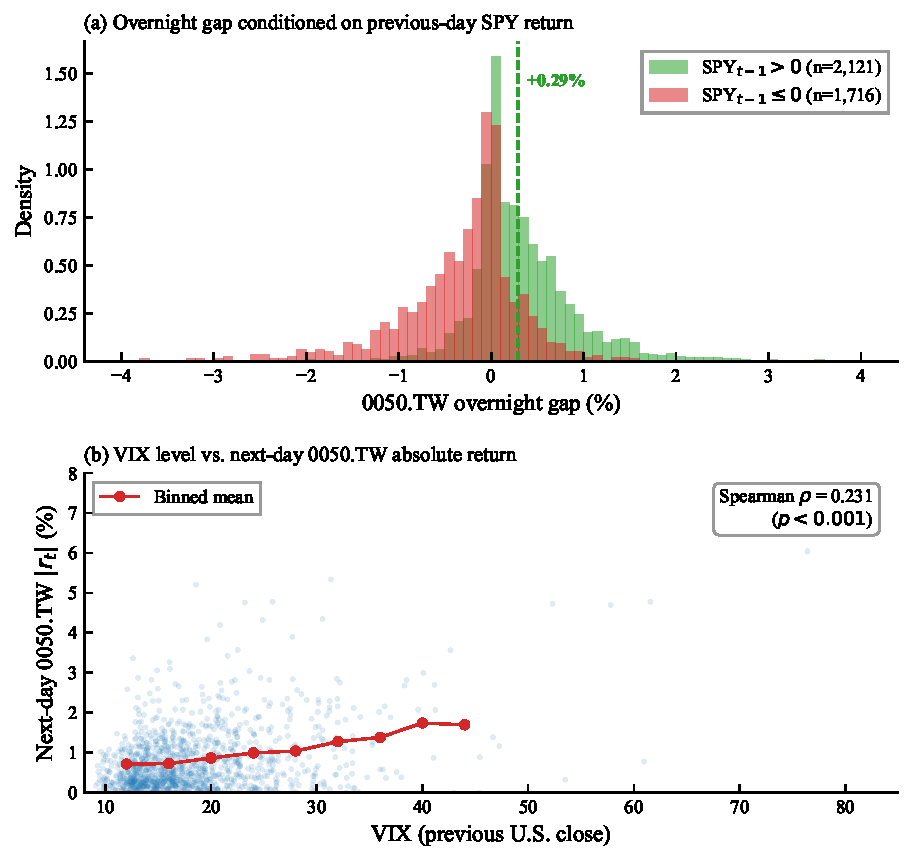
\includegraphics[width=0.95\textwidth]{figures/fig3_overnight_vix.pdf}
\caption{Information transmission from U.S.\ to Taiwan equity markets, 2010--2026. Panel~(a): Distribution of 0050.TW overnight gaps conditioned on the sign of the previous day's SPY close-to-close return. Panel~(b): VIX level versus next-day 0050.TW absolute return. Red circles show binned means.}
\label{fig:overnight_vix}
\end{figure}

\subsection{Identification: Time-Zone Gap, Not Factor Exposure}

We confirm that the cross-market predictability reflects genuine information transmission rather than common factor exposure using three tests: (1) the iShares MSCI Taiwan ETF (EWT), which trades on the NYSE during U.S. hours, fails to achieve statistical significance ($t < 1.96$), confirming the alpha originates from the time-zone gap; (2) European close-to-U.S.-open signals show a negative correlation ($r = -0.07$), consistent with the zero-overlap requirement; and (3) India and Indonesia controls both fail the $t > 3.0$ threshold.

\subsection{Robustness}

The c2c information transmission channel is robust to: multi-period out-of-sample tests (positive Sharpe in all five sub-periods, combined $t = 4.47$--$4.60$), block bootstrap (95\% CI $[0.65, \, 2.24]$, excluding zero), Bonferroni correction (six markets, adjusted threshold $t > 3.3$; all six pass on c2c basis), transaction cost sensitivity (breakeven $>3\%$ per switch for c2c), and lookback sensitivity (5-day and 10-day both exceed Harvey threshold on c2c). On an o2o basis, none of the individual markets pass the Bonferroni-adjusted threshold, underscoring the gap between information content and implementable alpha.

\subsection{ETFs Versus Individual Stocks}

The time-zone momentum strategy performs more consistently on the 0050.TW ETF than on individual Taiwanese stocks. Of the securities tested, four pass the \citet{harvey2016} $t > 3.0$ threshold on a c2c basis: 0056.TW ($t = 3.44$), Hon Hai ($t = 3.40$), 0050.TW ($t = 3.25$), and Cathay Financial ($t = 3.06$). ETFs offer a more stable substrate because diversification smooths idiosyncratic noise and the ETF mechanically reflects the broad market's response to U.S. information.
